\chapter{The Microscope}\label{the-microscope}

A \href{https://en.wikipedia.org/wiki/Microscope}{microscope} (from the
Ancient Greek: mikrós, ``small'' and skopeîn, ``to look'' or ``see'') is
an instrument used to see objects that are too small to be seen by the
naked eye. Microscopic means invisible to the eye unless aided by a
microscope.

There are many types of microscopes, and they may be grouped in
different ways. One way is to describe the way the instruments interact
with a sample to create images, either by sending a beam of light or
electrons to a sample in its optical path, or by scanning across, and a
short distance from, the surface of a sample using a probe. The most
common microscope (and the first to be invented) is the
\href{https://en.wikipedia.org/wiki/Optical_microscope}{optical
microscope}, which uses light to pass through a sample to produce an
image.

The objective lens of a microscope (Figure \ref{fig:objectives}) is a
cylinder containing one or more lenses that are typically made of glass.
It is essentially a high-powered magnifying glass which is brought very
close to the specimen being examined. The objective collects light from
the sample so that it comes to a focus inside the microscope tube. This
creates an enlarged image of the specimen.

\begin{figure}

{\centering 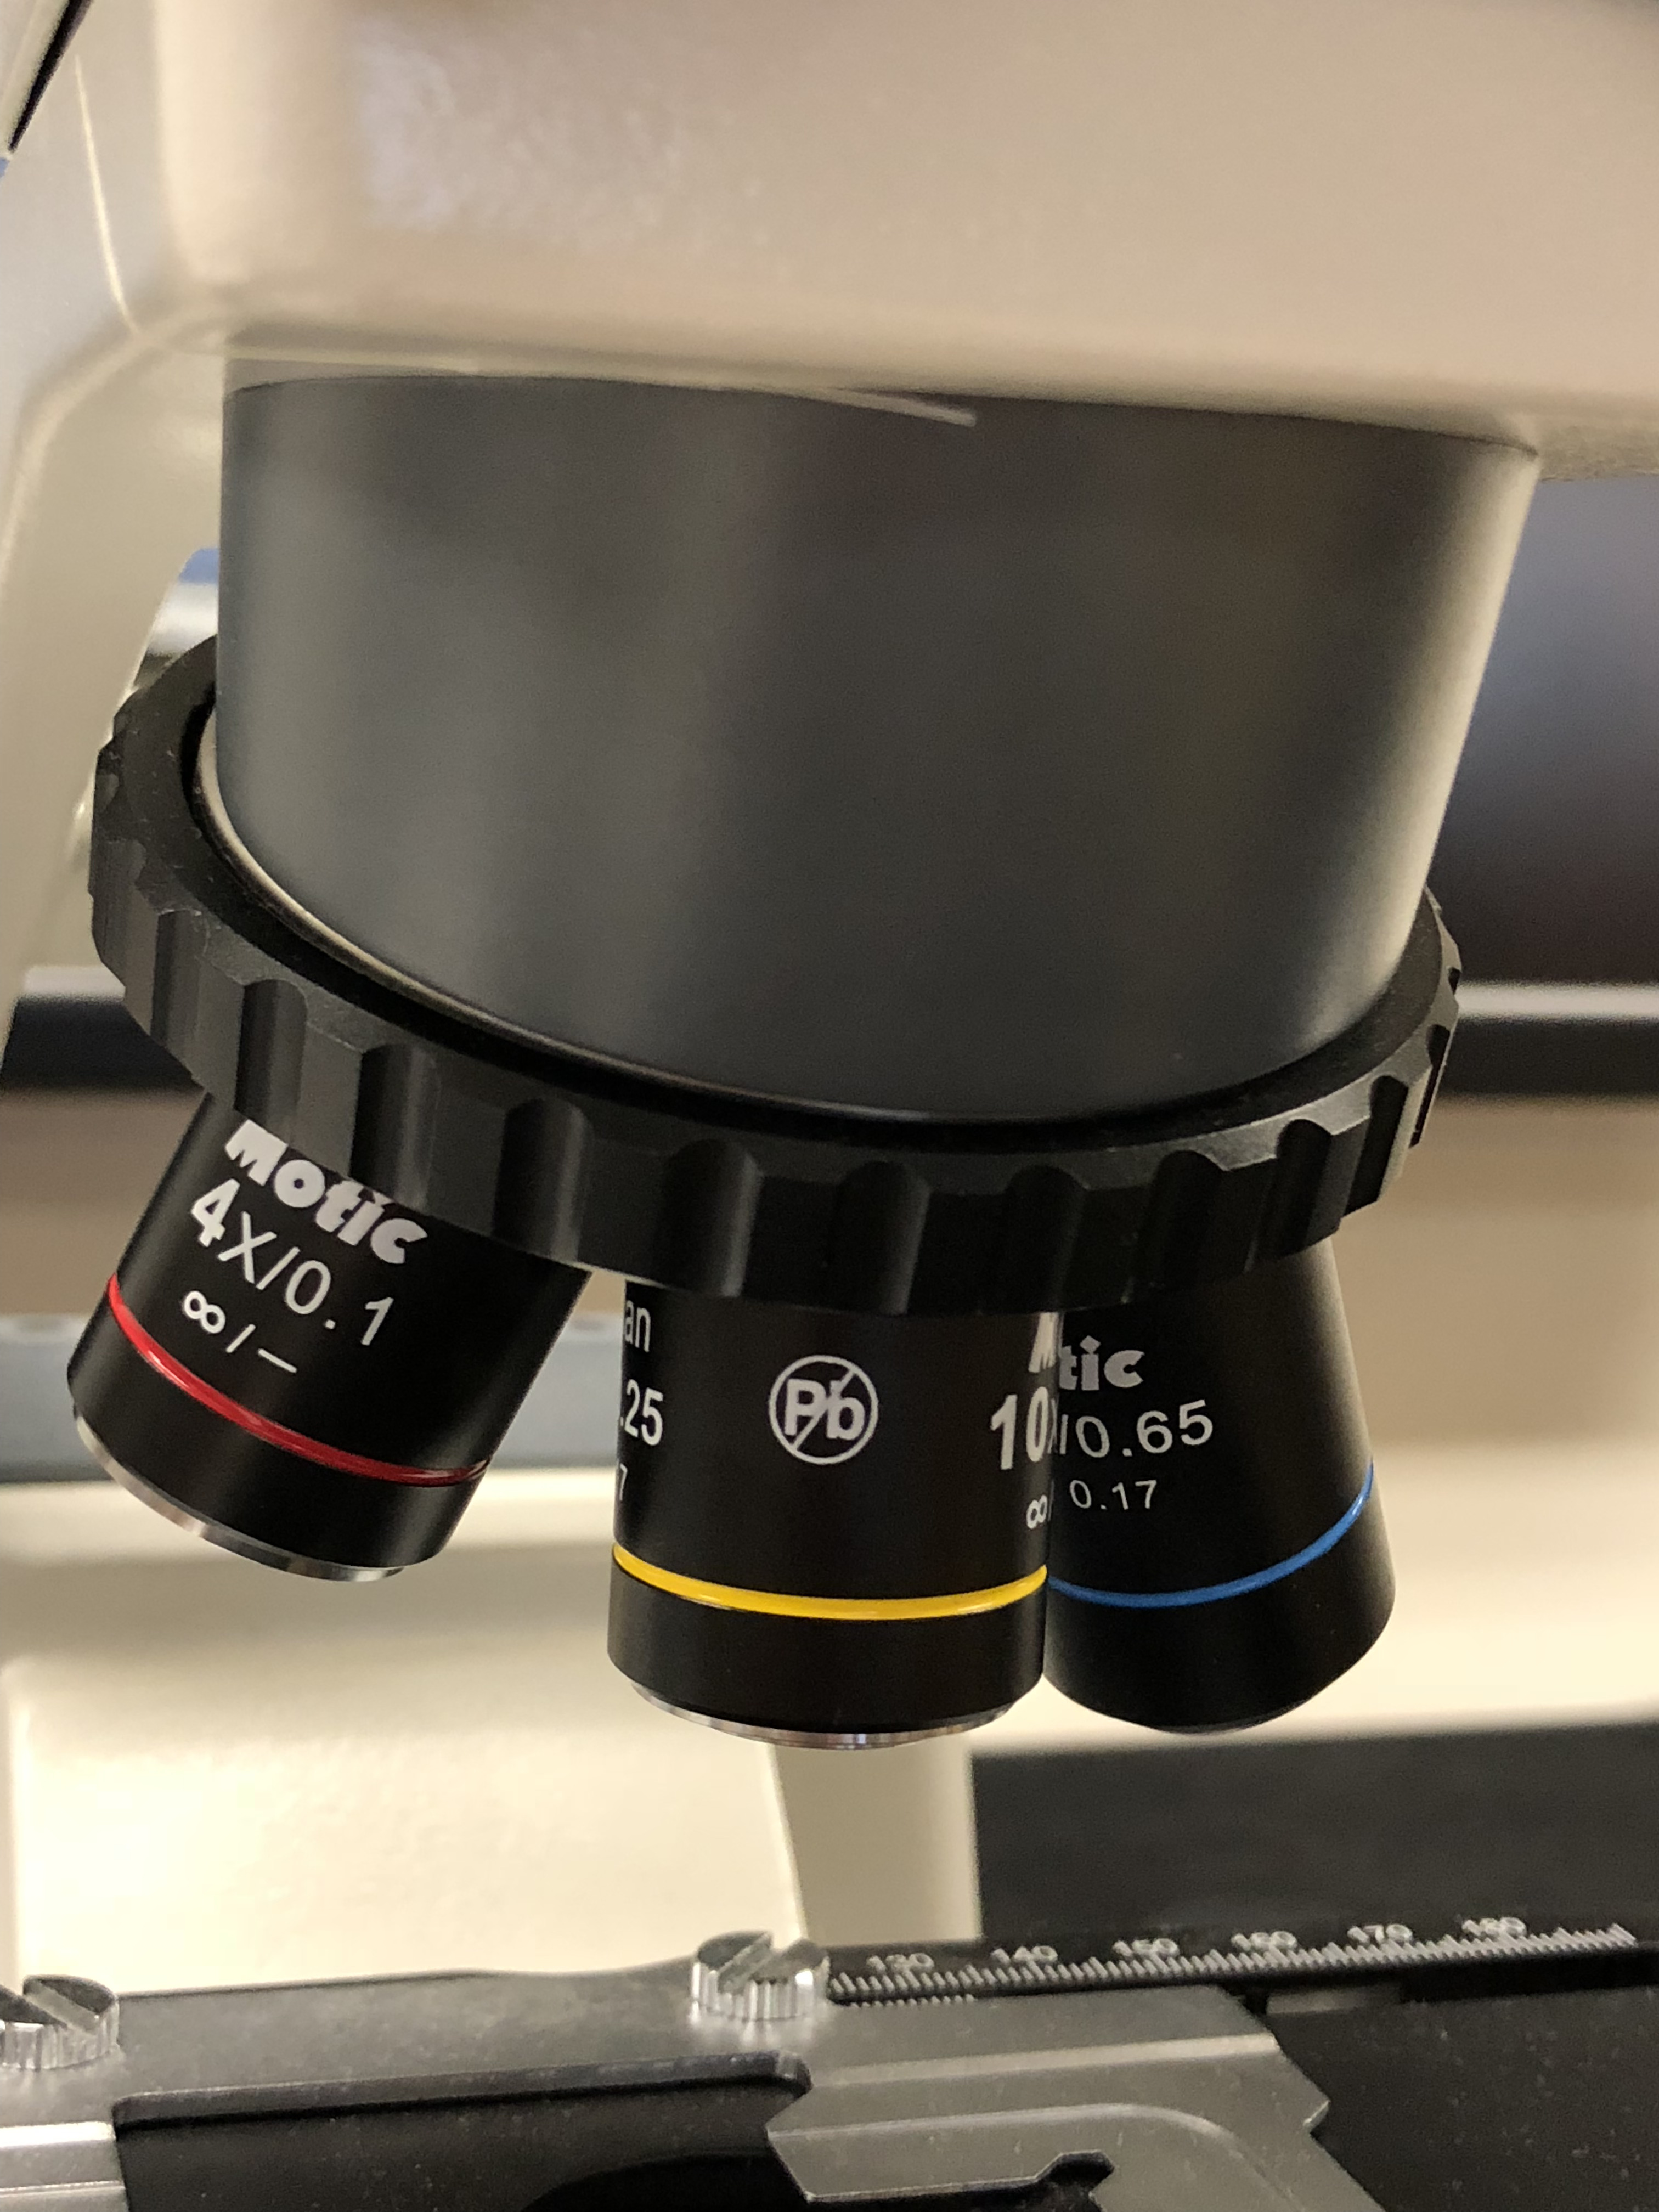
\includegraphics[width=0.7\linewidth]{./figures/microscope/Microscope_objectives}

}

\caption{The microscope objectives.}\label{fig:objectives}
\end{figure}

The eyepieces, or ocular lenses (Figure \ref{fig:oculars}), are the
lenses that are closest to your eyes when you look through the
microscope. The objective lens or mirror collects light and brings it to
focus creating an image. The eyepiece is placed near the focal point of
the objective to magnify this image. This image is inverted and can be
seen by removing the eyepiece and placing a piece of tracing paper over
the end of the tube. By carefully focusing a brightly lit specimen, a
highly enlarged image can be seen. It is this real image that is viewed
by the eyepiece lens that provides further enlargement. The amount of
magnification depends on the focal length of the eyepiece. The ocular in
our microscopes have a 0× magnification.

\begin{figure}

{\centering 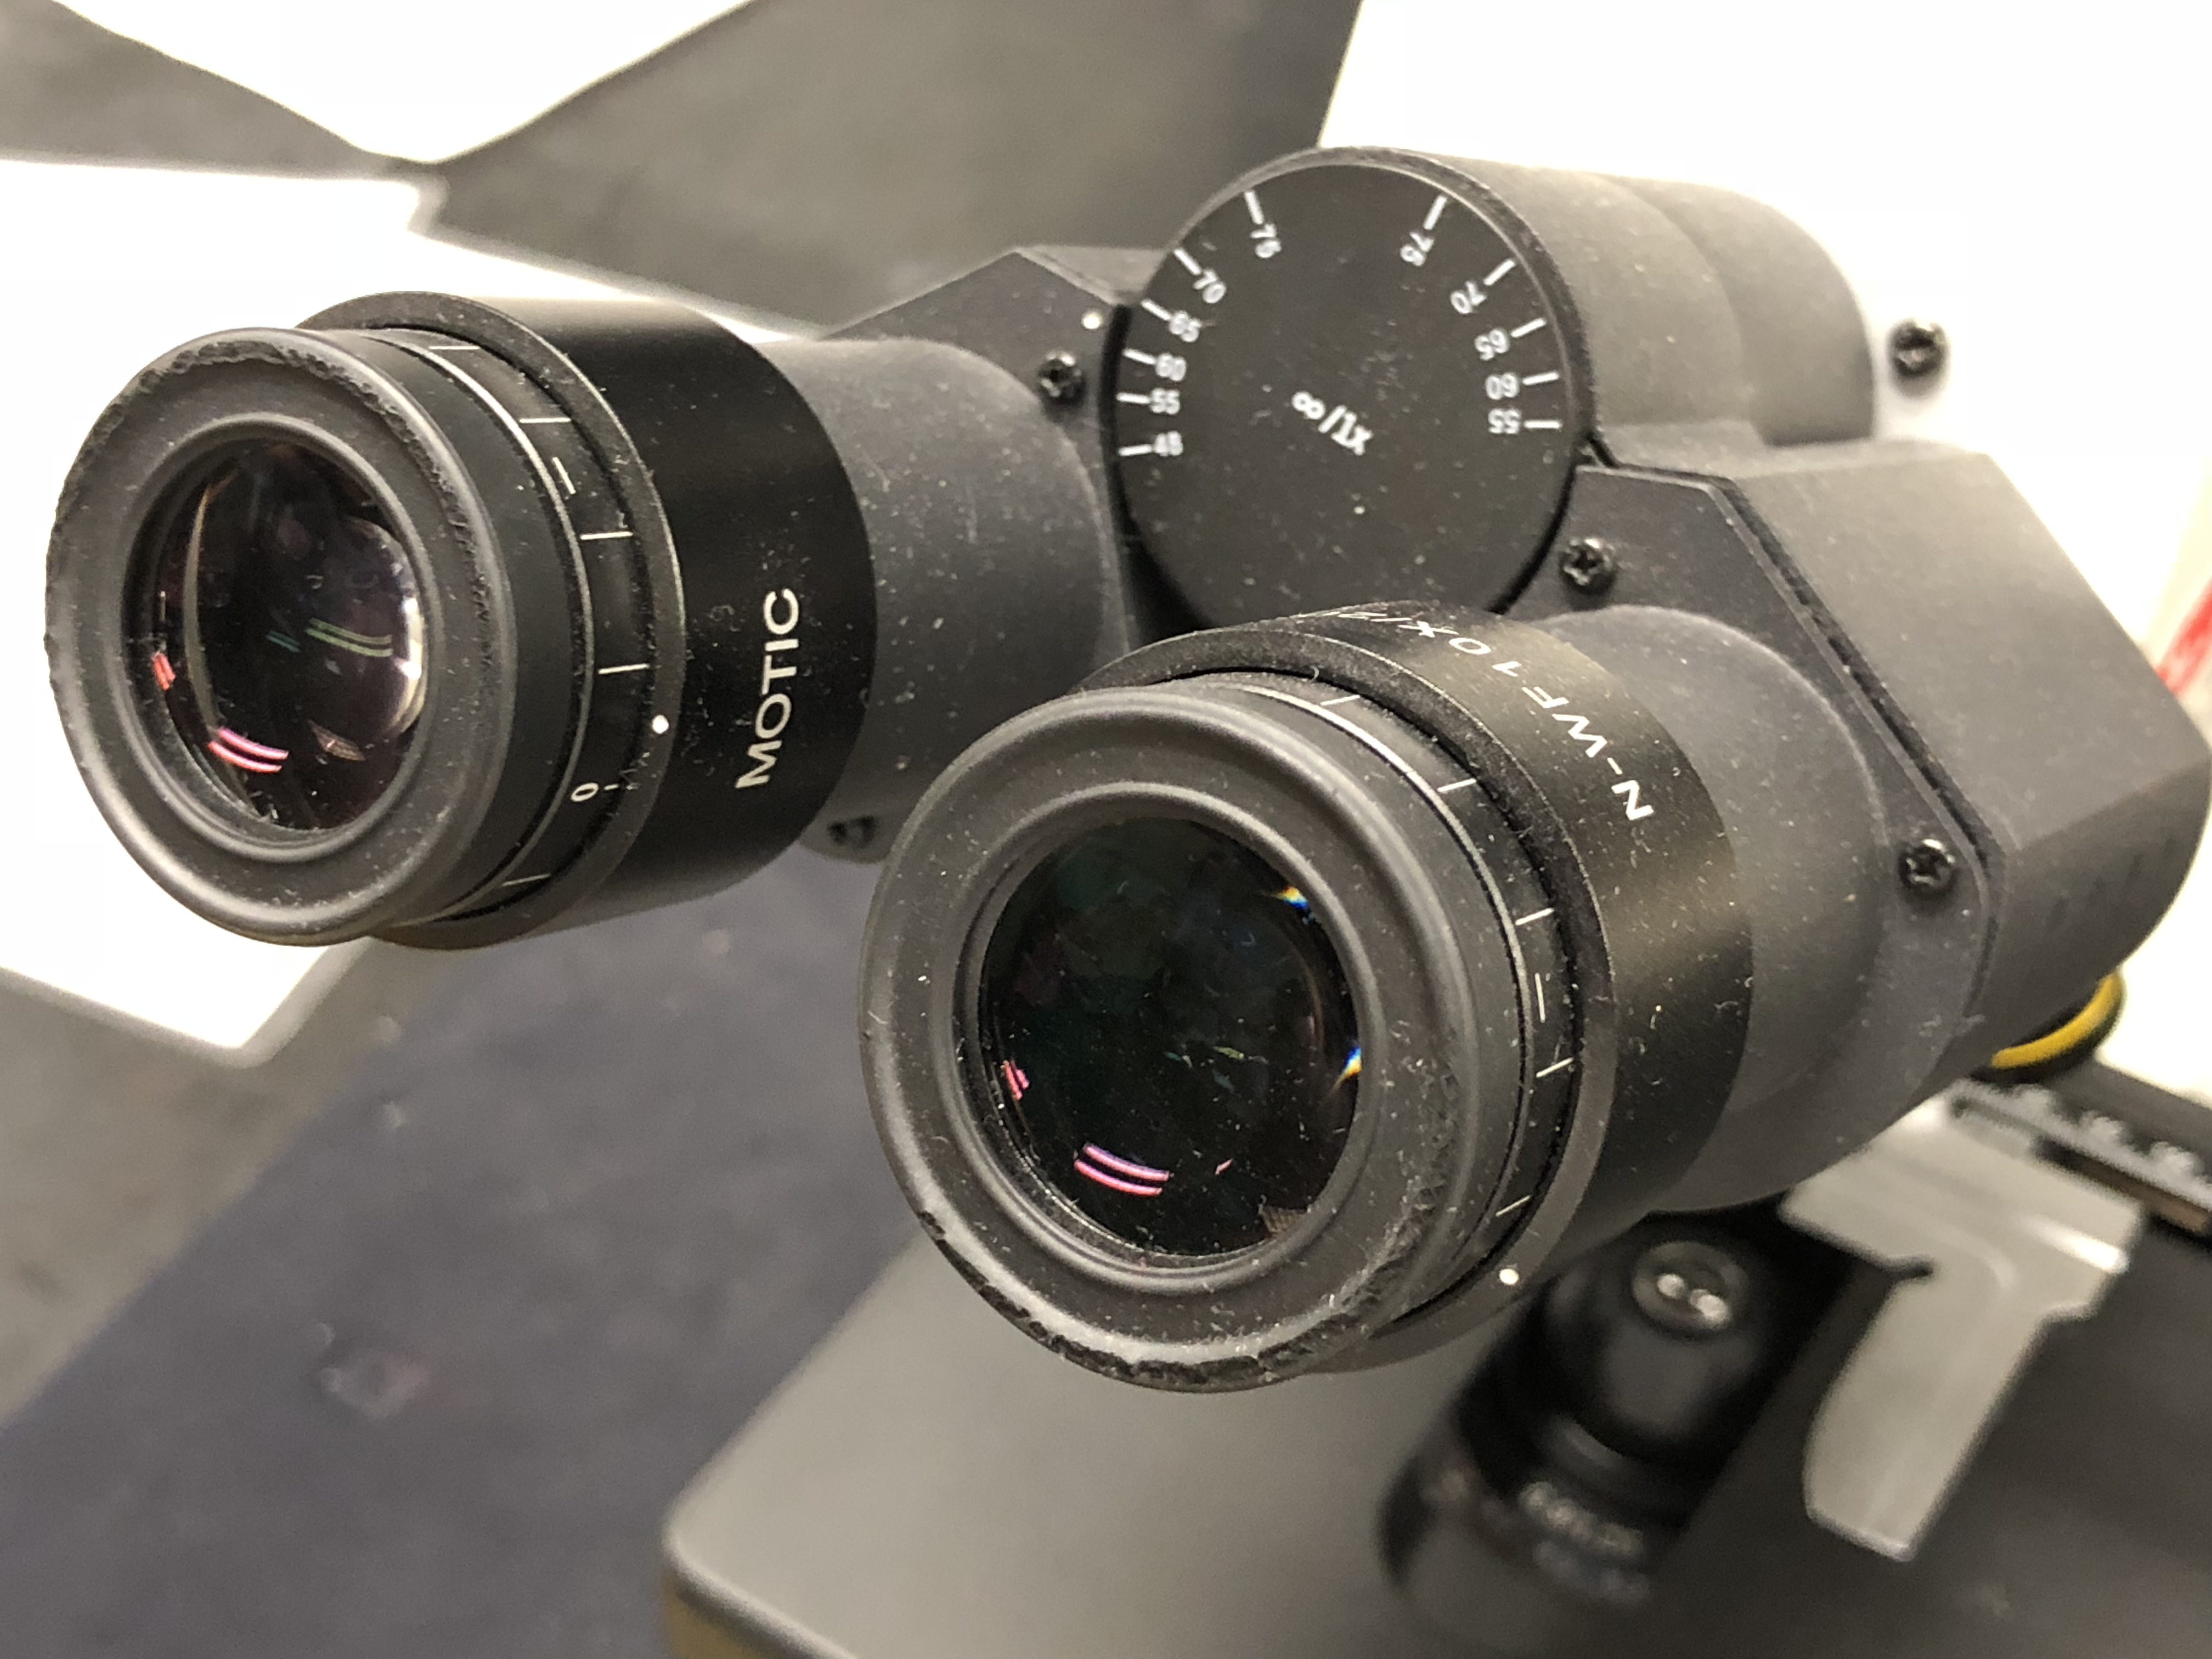
\includegraphics[width=0.7\linewidth]{./figures/microscope/Oculars}

}

\caption{The oculars (eye pieces) of the microscope.}\label{fig:oculars}
\end{figure}

Our microscopes have four objective lenses with different
magnifications, screwed into the circular ``nosepiece'' which you rotate
to select the required lens. These lenses are color coded for easier
use. The least powerful lens is called the scanning objective lens and
is a 4× objective. The second lens is referred to as the small objective
lens and is 10× lens. The most powerful lens out of the four are
referred to as the large objective lenses and are 40× and 100×. The 100×
objective is an oil-immersion lens. This objective is specially designed
for use with refractive index matching oil, which must fill the gap
between the objective lens and the specimen.

\begin{figure}

{\centering 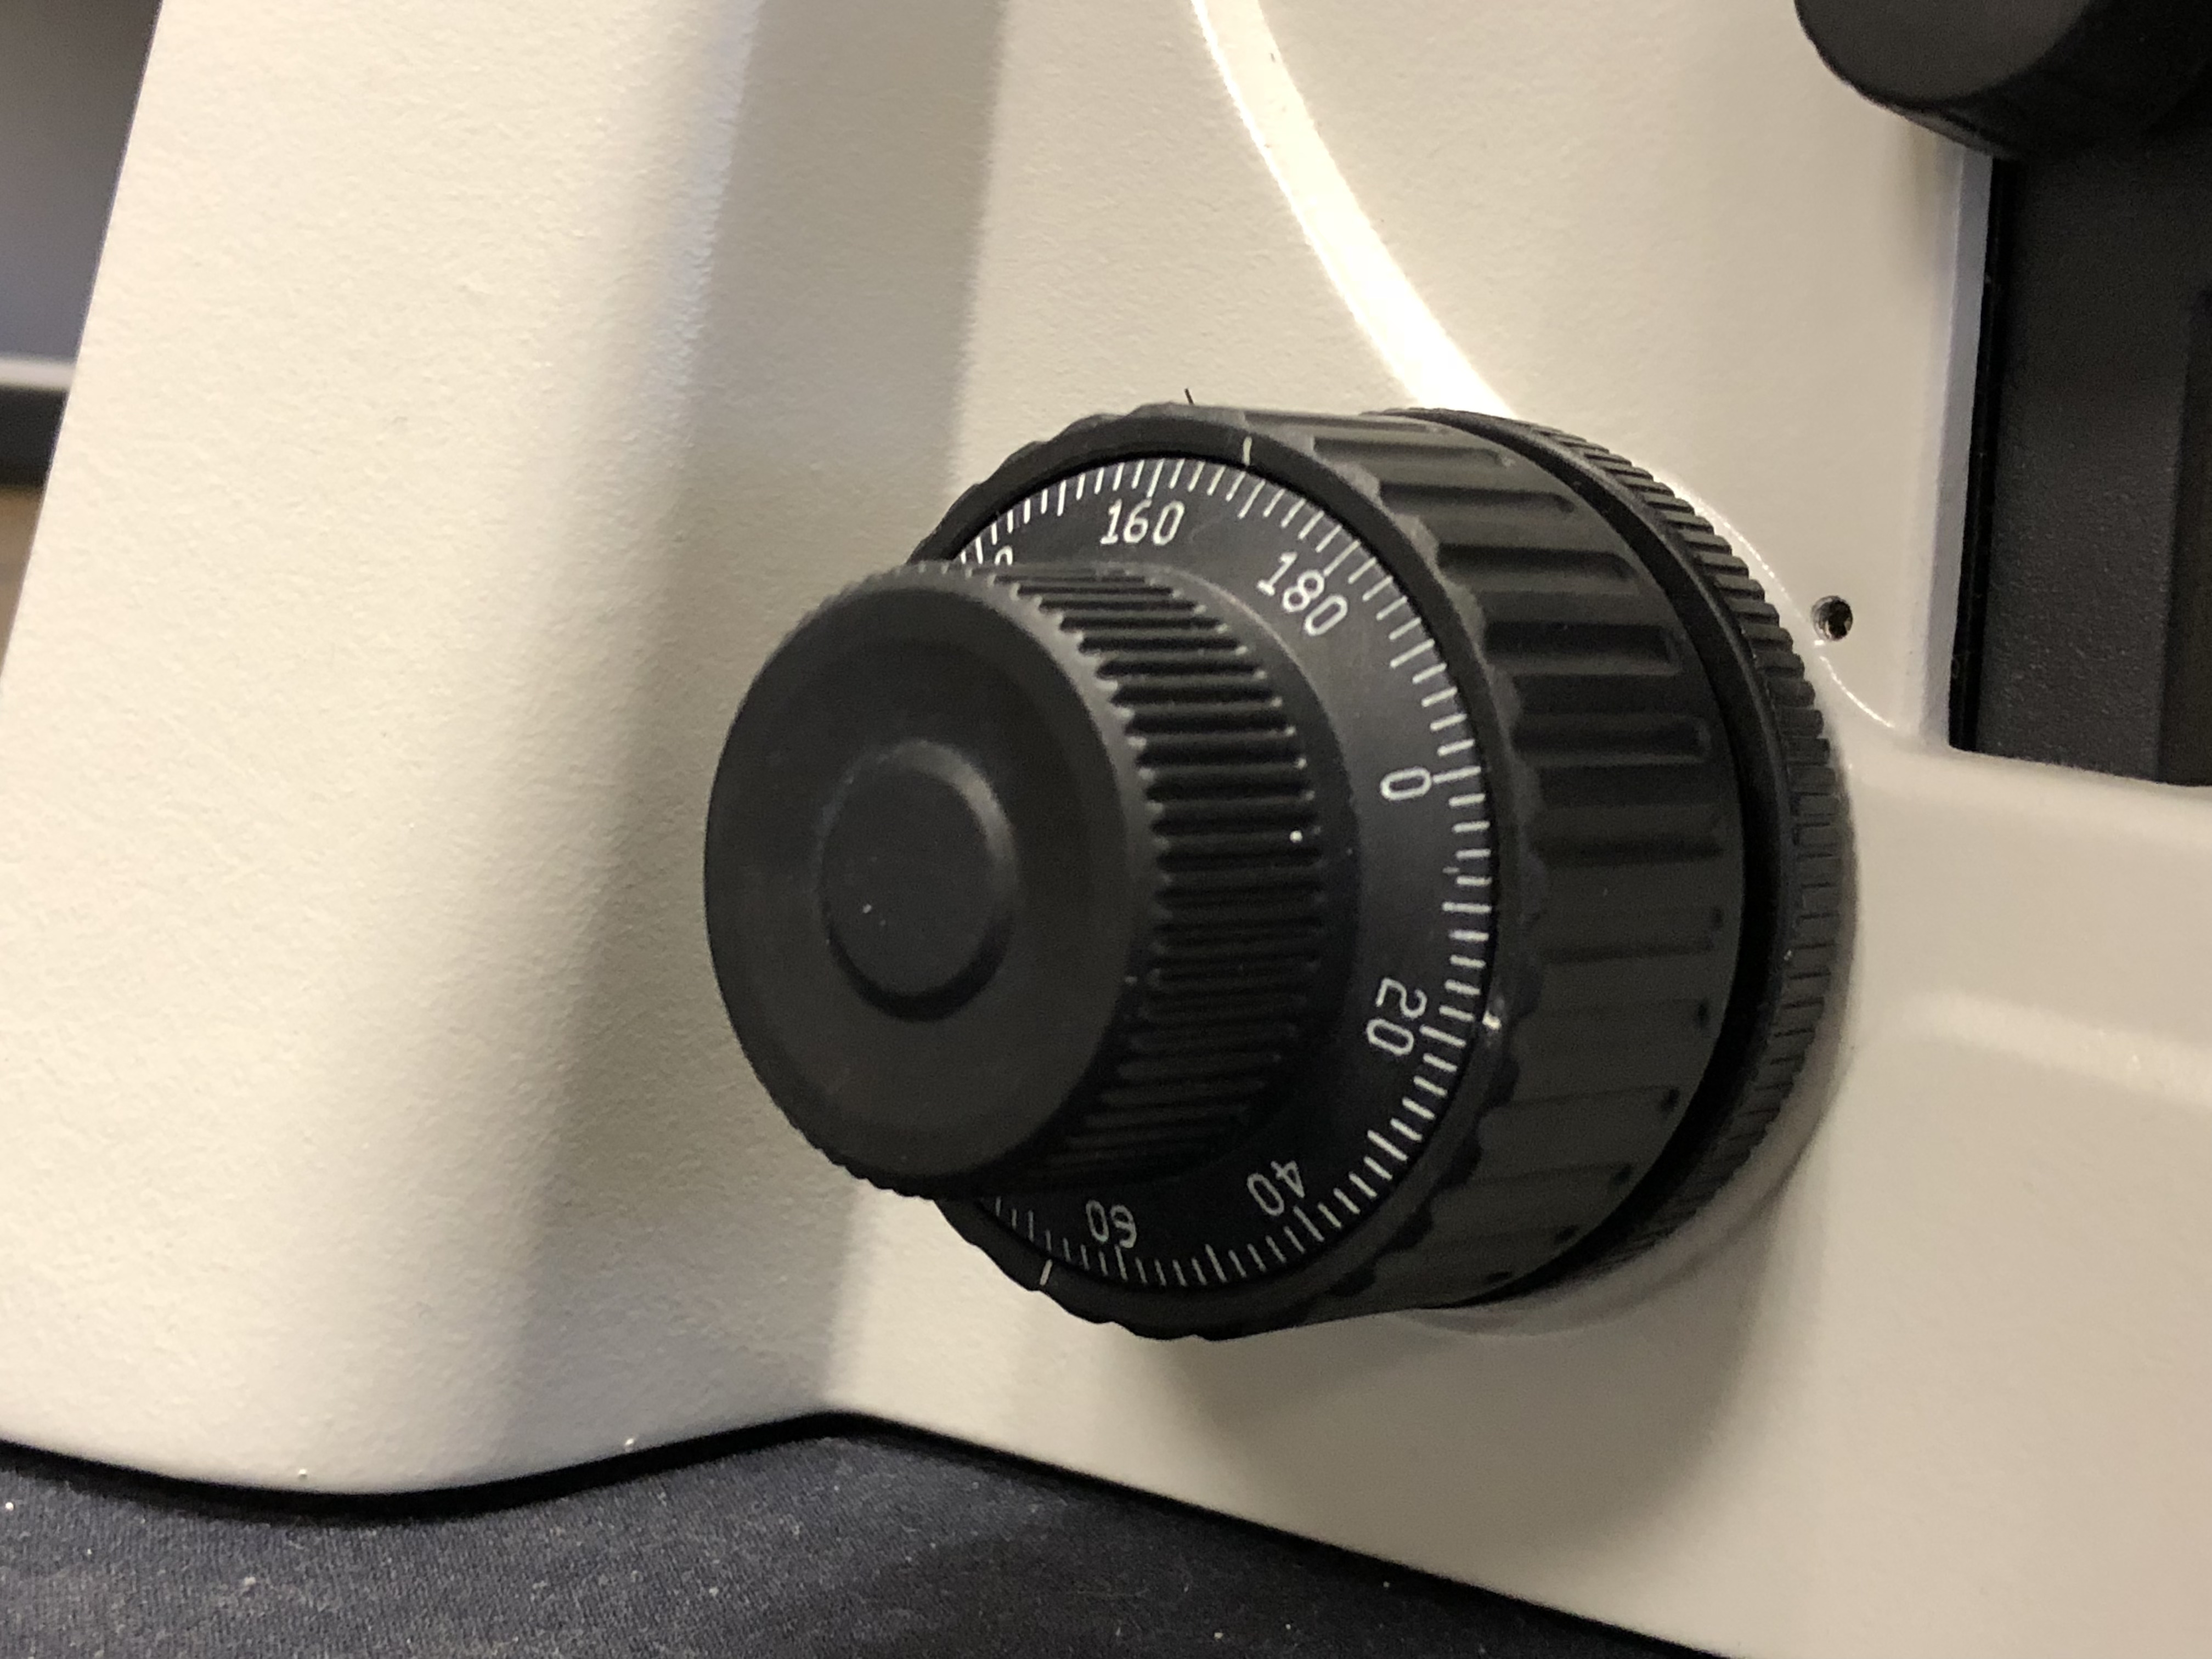
\includegraphics[width=0.7\linewidth]{./figures/microscope/focus}

}

\caption{The coarse (big wheel) and fine (small wheel) focus adjustment knobs.}\label{fig:focus}
\end{figure}

The stage is a platform below the objective which supports the specimen
being viewed. Adjustment knobs (on the left side of the microscope) move
the stage up and down with separate adjustment for coarse and fine
focusing (Figure \ref{fig:focus}). In the center of the stage is a hole
through which light passes to illuminate the specimen (Figure
\ref{fig:stage}). The stage has arms to hold slides (rectangular glass
plates on which the specimen is mounted).

\begin{figure}

{\centering 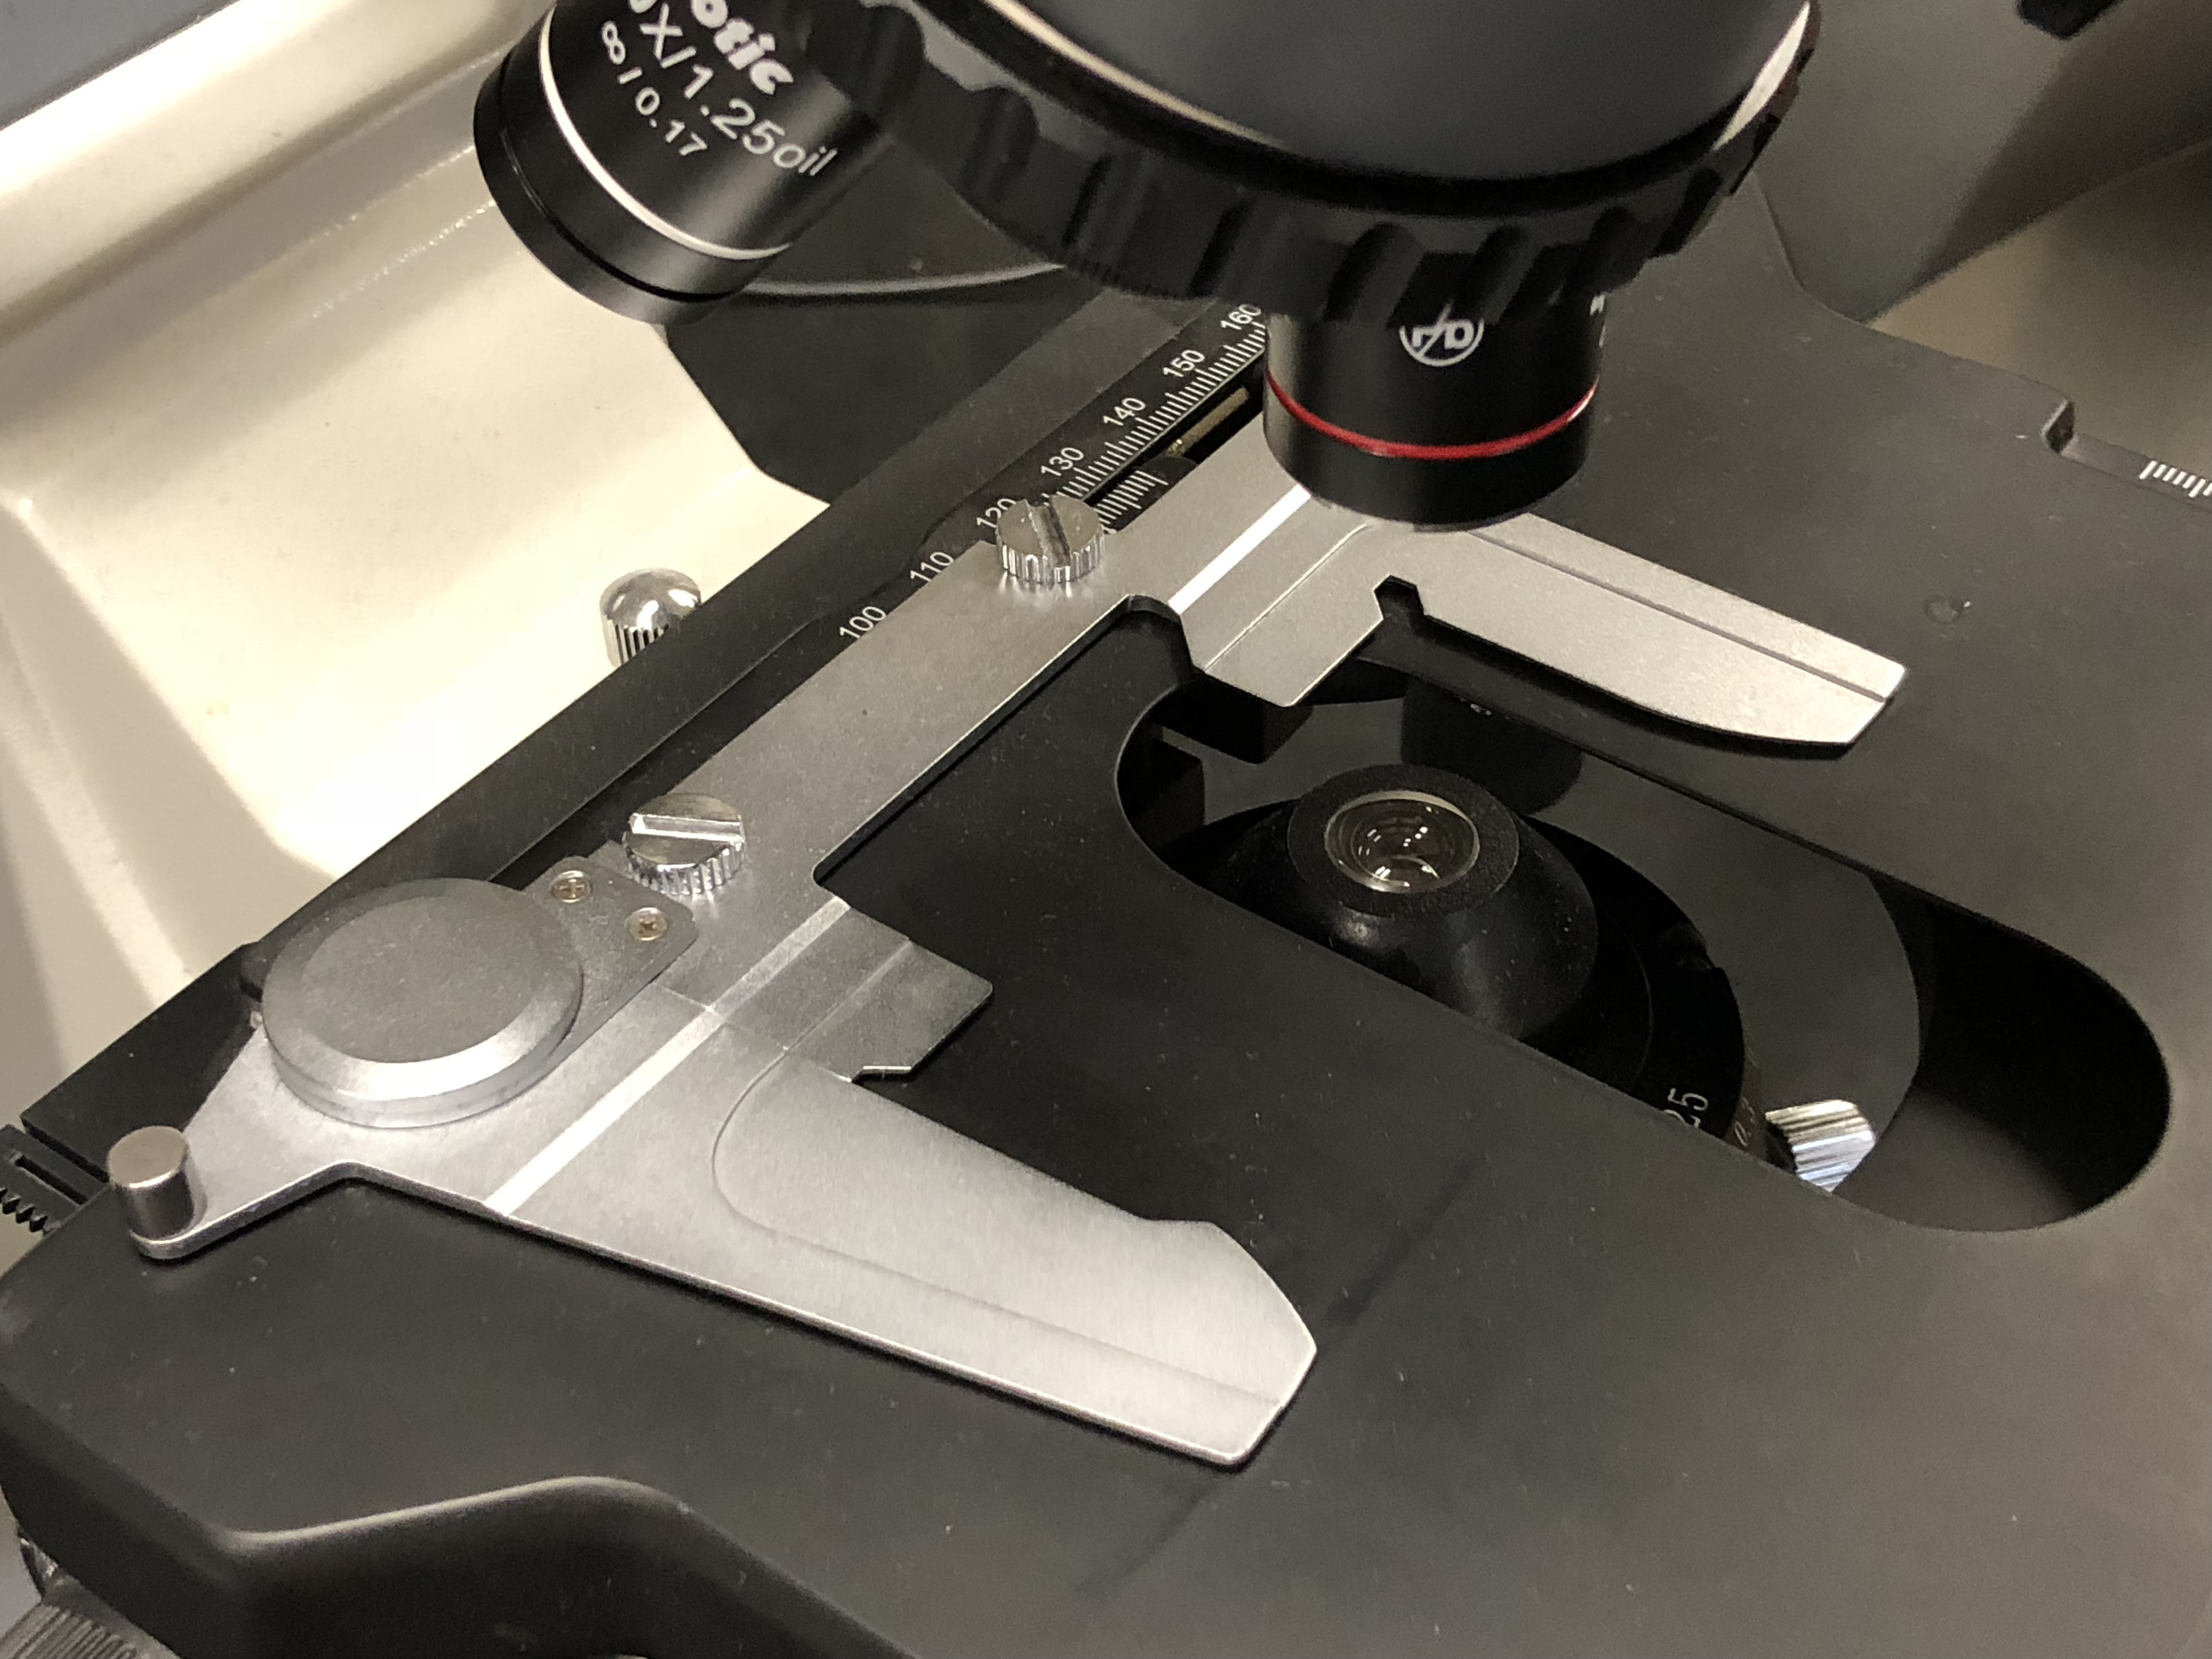
\includegraphics[width=0.7\linewidth]{./figures/microscope/stage}

}

\caption{The stage with the slide holder and central opening showing the condenser lens.}\label{fig:stage}
\end{figure}

The stage moves up and down for focus. Always start with the lowest
magnification in order to center the specimen on the stage. After moving
to a higher magnification re-focus using the fine focus knob. You may
also have to adjust the horizontal positions using the horizontal stage
and slide holder adjustment knobs hanging down on the right side of the
stage (Figure \ref{fig:condenser}). Our microscopes, an adjustable LEDs
light source (knob on the right side). The condenser is a lens designed
to focus light from the illumination source onto the sample. The light
source and condenser also each include a diaphragm to influence the
quality and intensity of the illumination. For our purposes, the
diaphragms should always be completely open. Adjust the light intensity
only using the knob on the right side of the frame of the microscope
(the black knob below the green switch in Figure \ref{fig:stage}.

\begin{figure}

{\centering 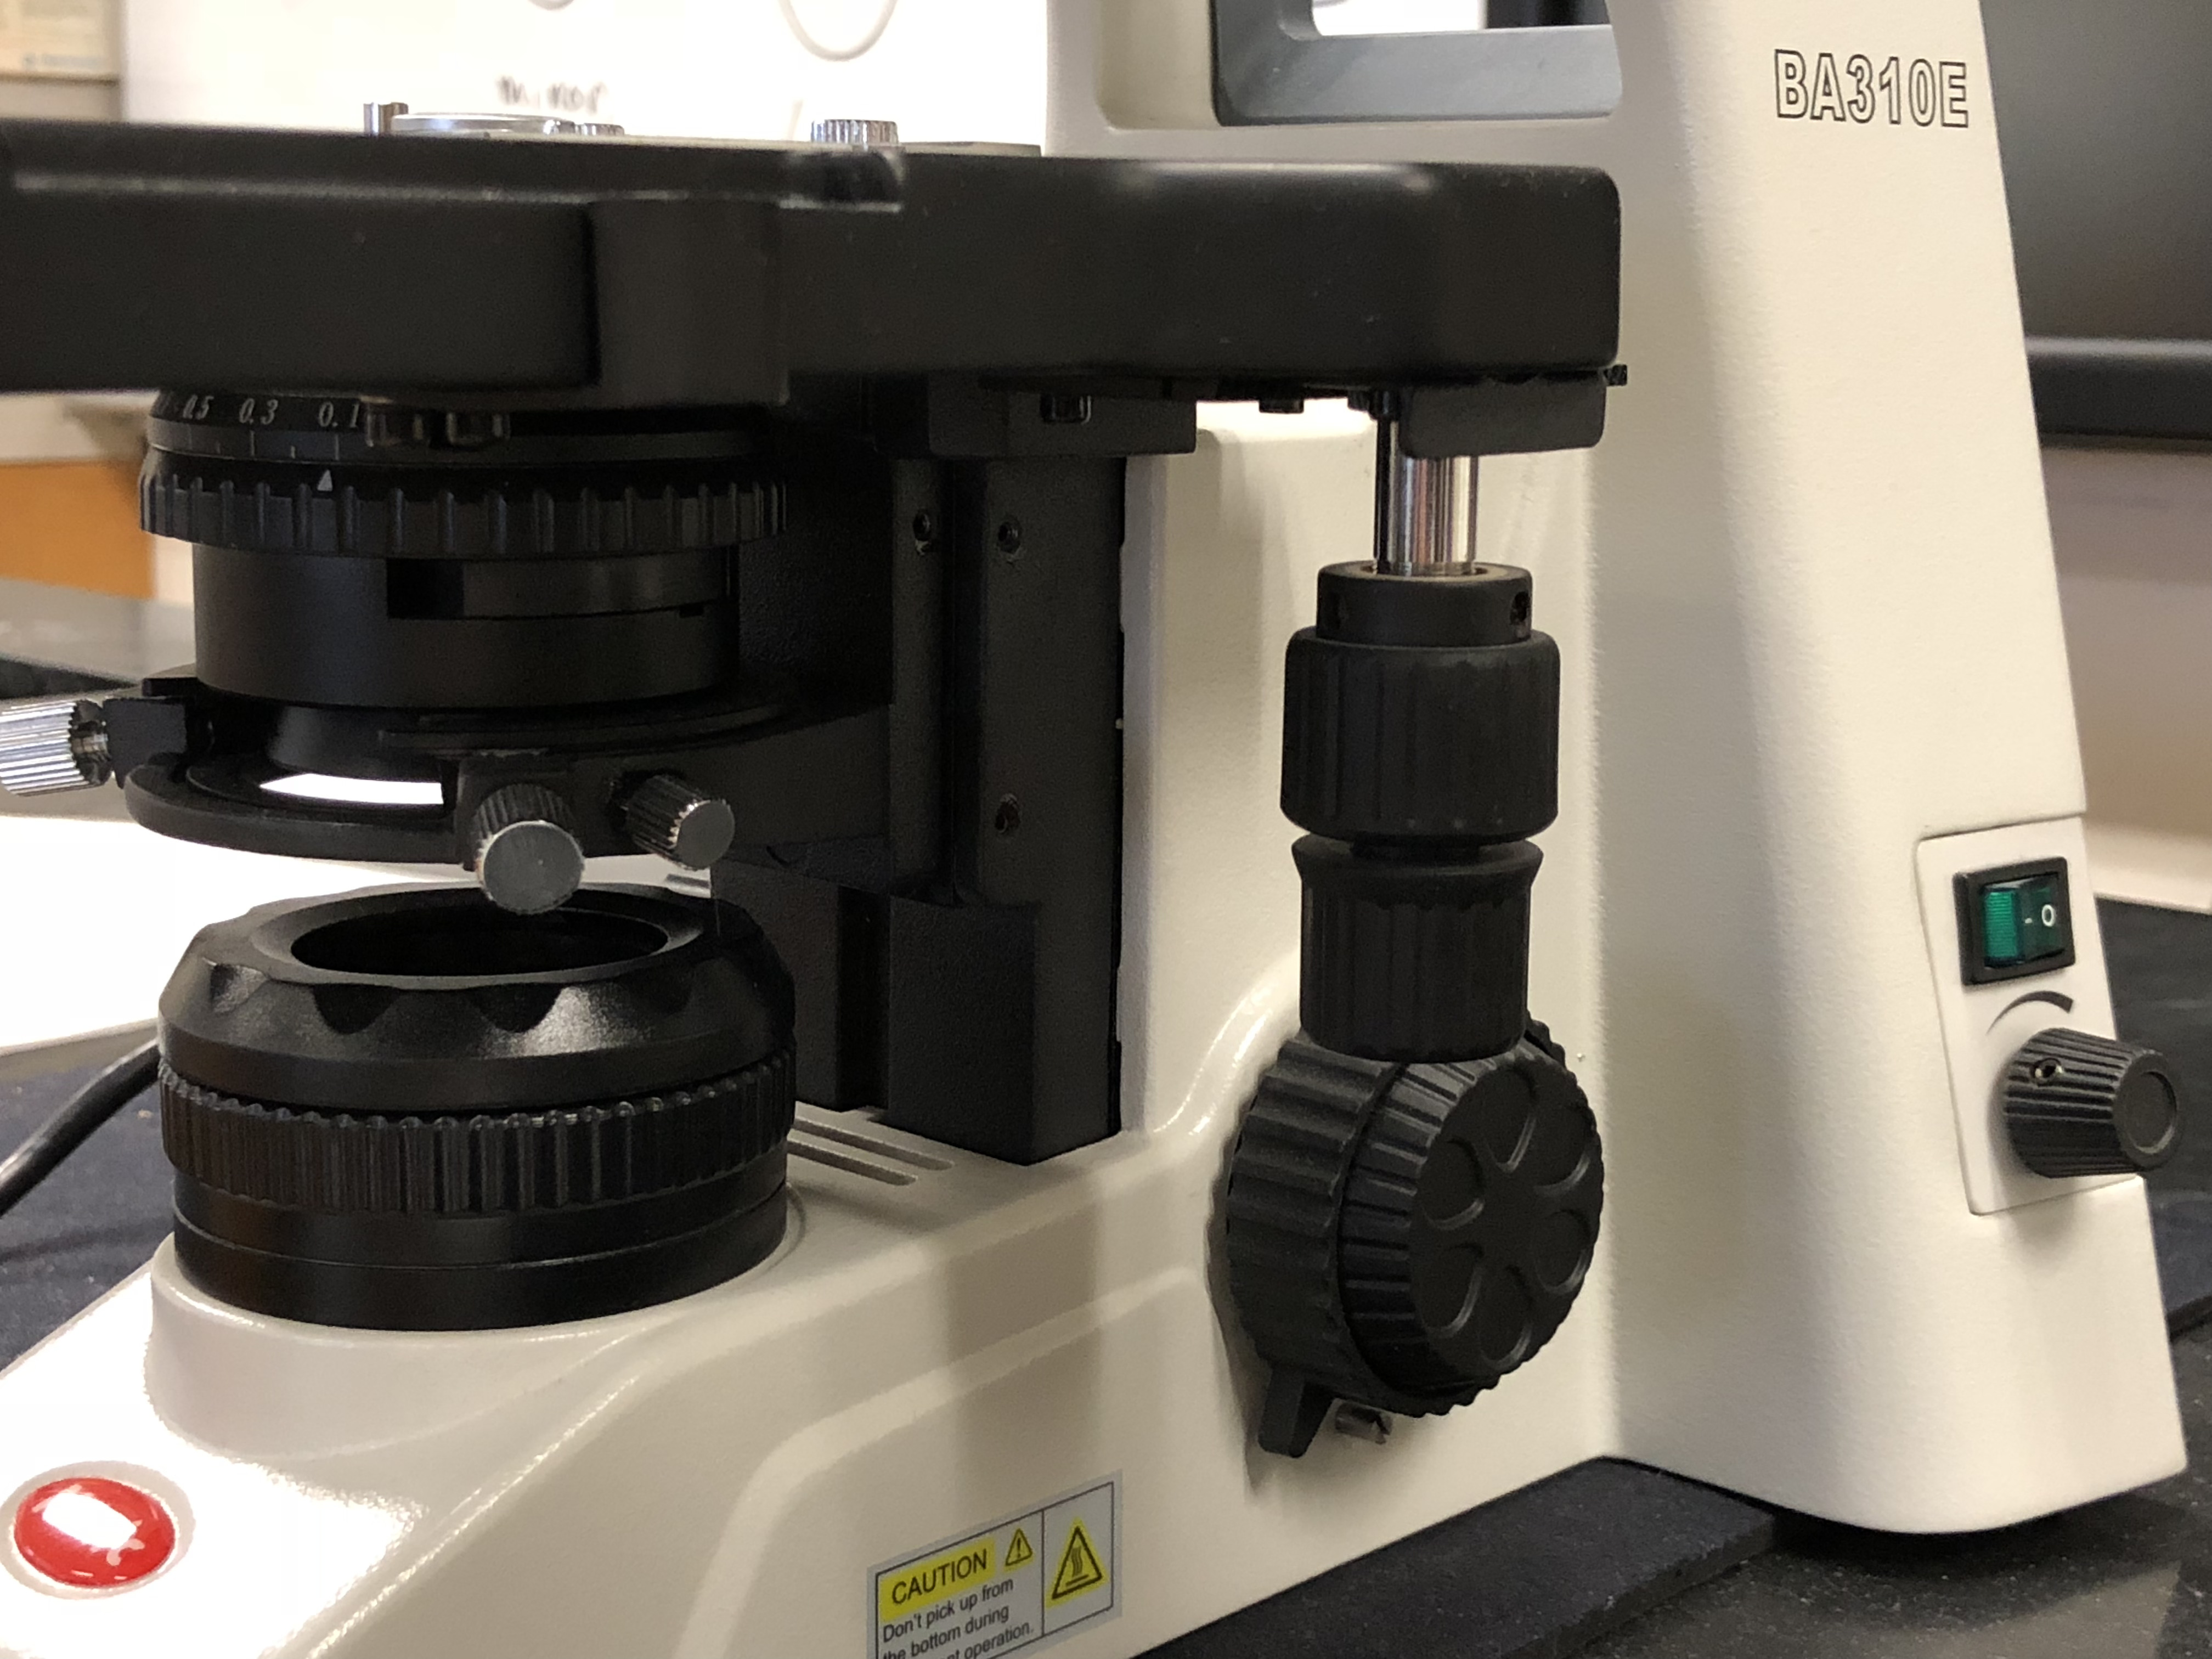
\includegraphics[width=0.7\linewidth]{./figures/microscope/condenser}

}

\caption{The condenser (below the stage), the horizontal stage and slide holder adjustment knobs (hanging down from the stage), the light on switch and light intensity adjustment knob (in the back).}\label{fig:condenser}
\end{figure}

We have prepared a number of videos that introduce our microscopes to
you and also demonstrate how you can capture images of the slides that
you are viewing and transfer them to your own equipment.

\section{How to turn on the
microscope}\label{how-to-turn-on-the-microscope}

The tablets and microscopes must be turned on in a specific order:

\begin{enumerate}
\def\labelenumi{\arabic{enumi}.}
\tightlist
\item
  Microscope must be plugged in. If already plugged in, proceed to step
  3.
\item
  Motic logo will appear on tablet. After a few seconds, the charging
  symbol appears.
\item
  Press and hold the power button on the tablet for 6 seconds.
\item
  Motic symbol will appear again and tablet will start up.
\item
  Turn on microscope using the switch on the lower right side.
\end{enumerate}

\section{View Prepared Slides}\label{view-prepared-slides}

\begin{enumerate}
\def\labelenumi{\arabic{enumi}.}
\tightlist
\item
  Get a white slide box.
\item
  Clean all of the exposed lenses with special lens paper. Do not use
  paper towels, Kimwipes®, or cloth as this will scratch the lenses. If
  the view through the microscope becomes blurred, additional cleaning
  with lens paper may be necessary. Use alcohol pads if necessary.
\item
  Make sure that the low power objective is clicked into position.
\item
  Move the oculars as far apart from each other as possible then look
  through them with both eyes open. You will see two non-overlapping
  regions of light. Push the oculars slowly towards each other until you
  see one circle of light.
\item
  Always use both eyes when you look at slides. This will avoid eye
  strain and headaches.
\item
  Get the slide labelled ``Letter e'' (Figure \ref{fig:letter}) from the
  slide box.
\item
  Place the slide (coverslip up) on the stage and center the specimen
  over the opening in the stage.
\item
  Always start with the low power (4×) objective in place.
\item
  While looking through the ocular, use the coarse adjustment knob to
  slowly move the stage upward until the specimen comes into focus. If
  it does not, check to see that the material is centered on the stage,
  lower the stage, and try again.
\item
  Using the fine adjustment knob, obtain a sharp focus.
\item
  To increase the magnification, be sure the area you wish to examine
  specifically is in the center of the field; then, watching from the
  side to be sure that the objective clears the slide, turn the
  nose-piece until the next higher power objective clicks into position.
  The material now should be in view and should require only slight
  focusing with the fine adjustment. Never focus with the coarse
  adjustment under high power.
\item
  What happens when you increase the magnification?
\item
  Before removing the slide, always return the microscope to low power
  and turn the coarse adjustment knob until the stage is moved all the
  way down.
\item
  View the computer chip slide (Figure \ref{fig:chip}).
\item
  View the colored threads slide (Figure \ref{fig:threads}).
\item
  Which thread is at the bottom, in the middle, on top?
\item
  Depth perception requires that a slightly different angle of an object
  is seen by the left and right eye. This happens because of the
  horizontal separation parallax of the eyes. If an object is far away,
  the disparity of that image falling on both retinas will be small. If
  the object is close or near, the disparity will be large. The
  microscope presents the same view to both eyes. Therefore, the only
  way to answer the above question is to change the focus of the image
  and observe what happens: when you move the stage upwards, to bring
  the slide closer to the objective, the thread that is on top will come
  into focus first, the middle one second and the bottom one last. Try
  it and write down your answer!

  \begin{itemize}
  \tightlist
  \item
    Bottom thread: \underline{\phantom{answer}}
  \item
    Middle thread: \underline{\phantom{answer}}
  \item
    Top thread: \underline{\phantom{answer}}
  \end{itemize}
\item
  View the stage micrometer slide (Figure \ref{fig:scale}).
\item
  What is the unit of this scale?
\item
  What is the distance between 1.0 and 1.5 in meters?
\item
  How many subdivisions can you distinguish between 0 and 0.1?
\item
  What is the distance in meters between the smallest subdivision?
\item
  View the blood smear slide (Figure \ref{fig:smear}).
\item
  Which cells are red blood cells? Mark with an arrow and label it
  ``RBC''.
\item
  Which cells are white blood cells? Mark with an arrow and label it
  ``WBC''.
\item
  Return the slides to the slide boxes and the slide boxes to the bench
  where you picked it up.
\end{enumerate}

\begin{figure}

{\centering 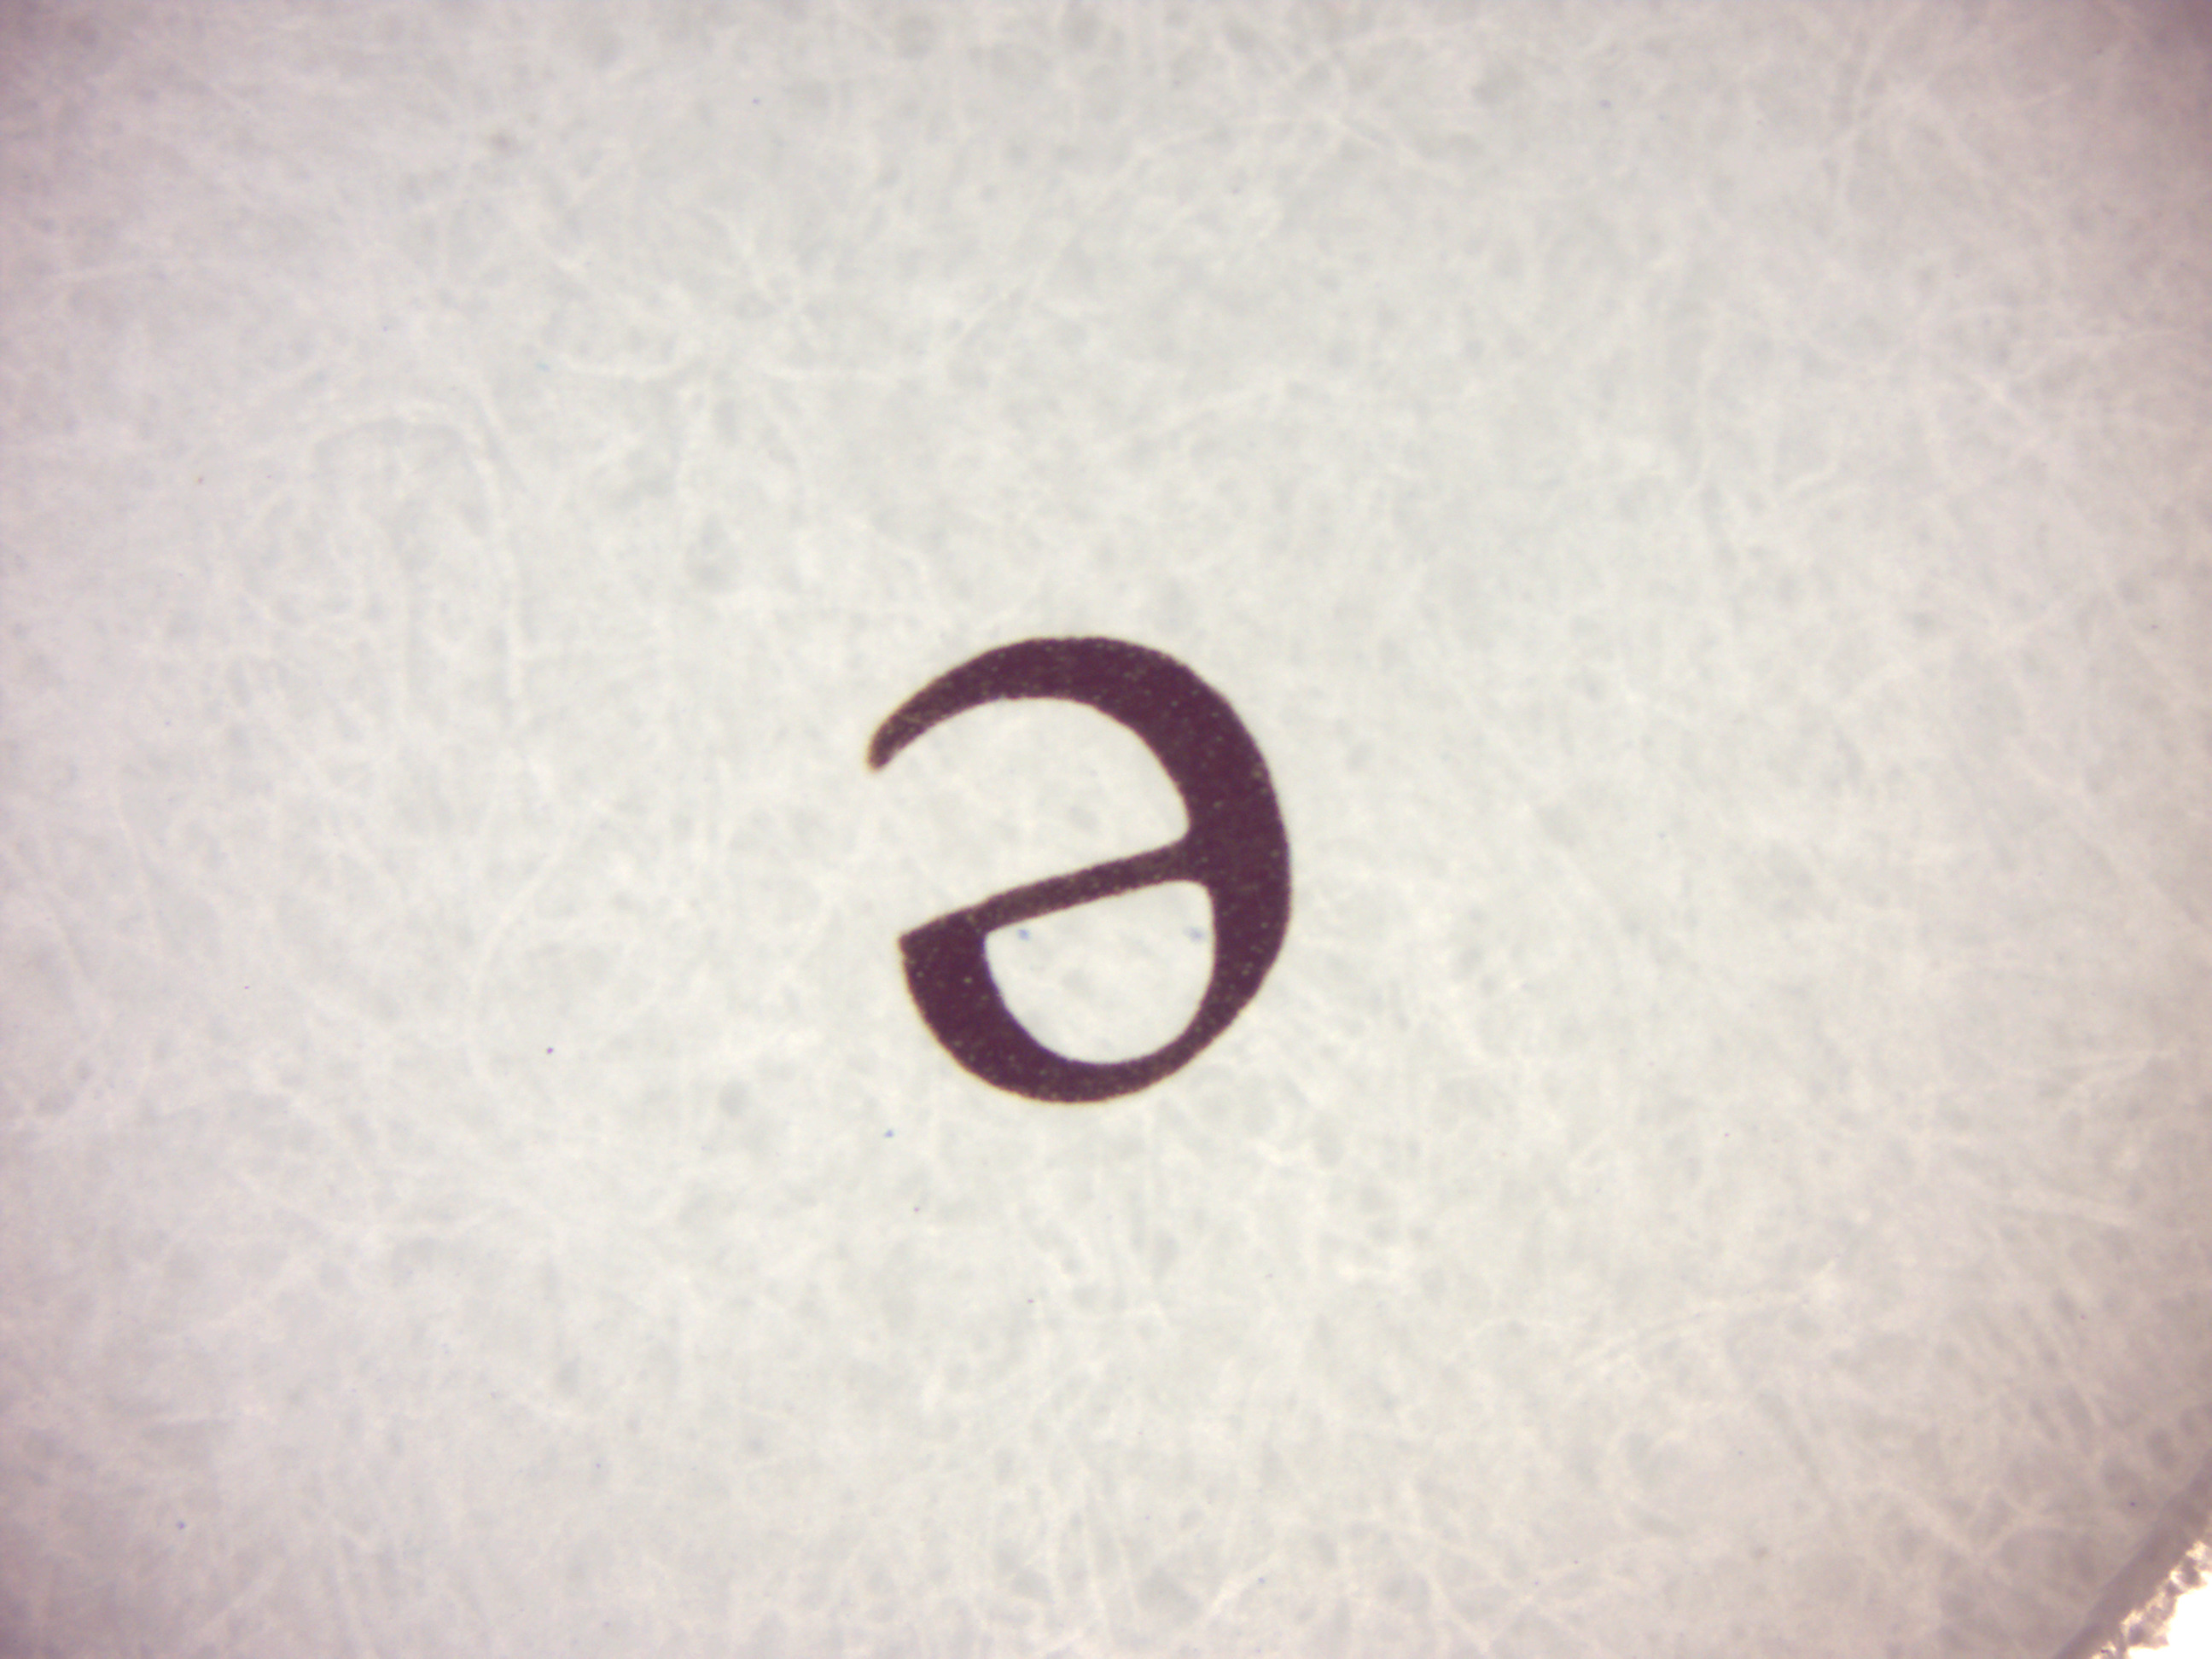
\includegraphics[width=0.7\linewidth]{./figures/microscope/Letter_e}

}

\caption{A printed letter.}\label{fig:letter}
\end{figure}

\begin{figure}

{\centering 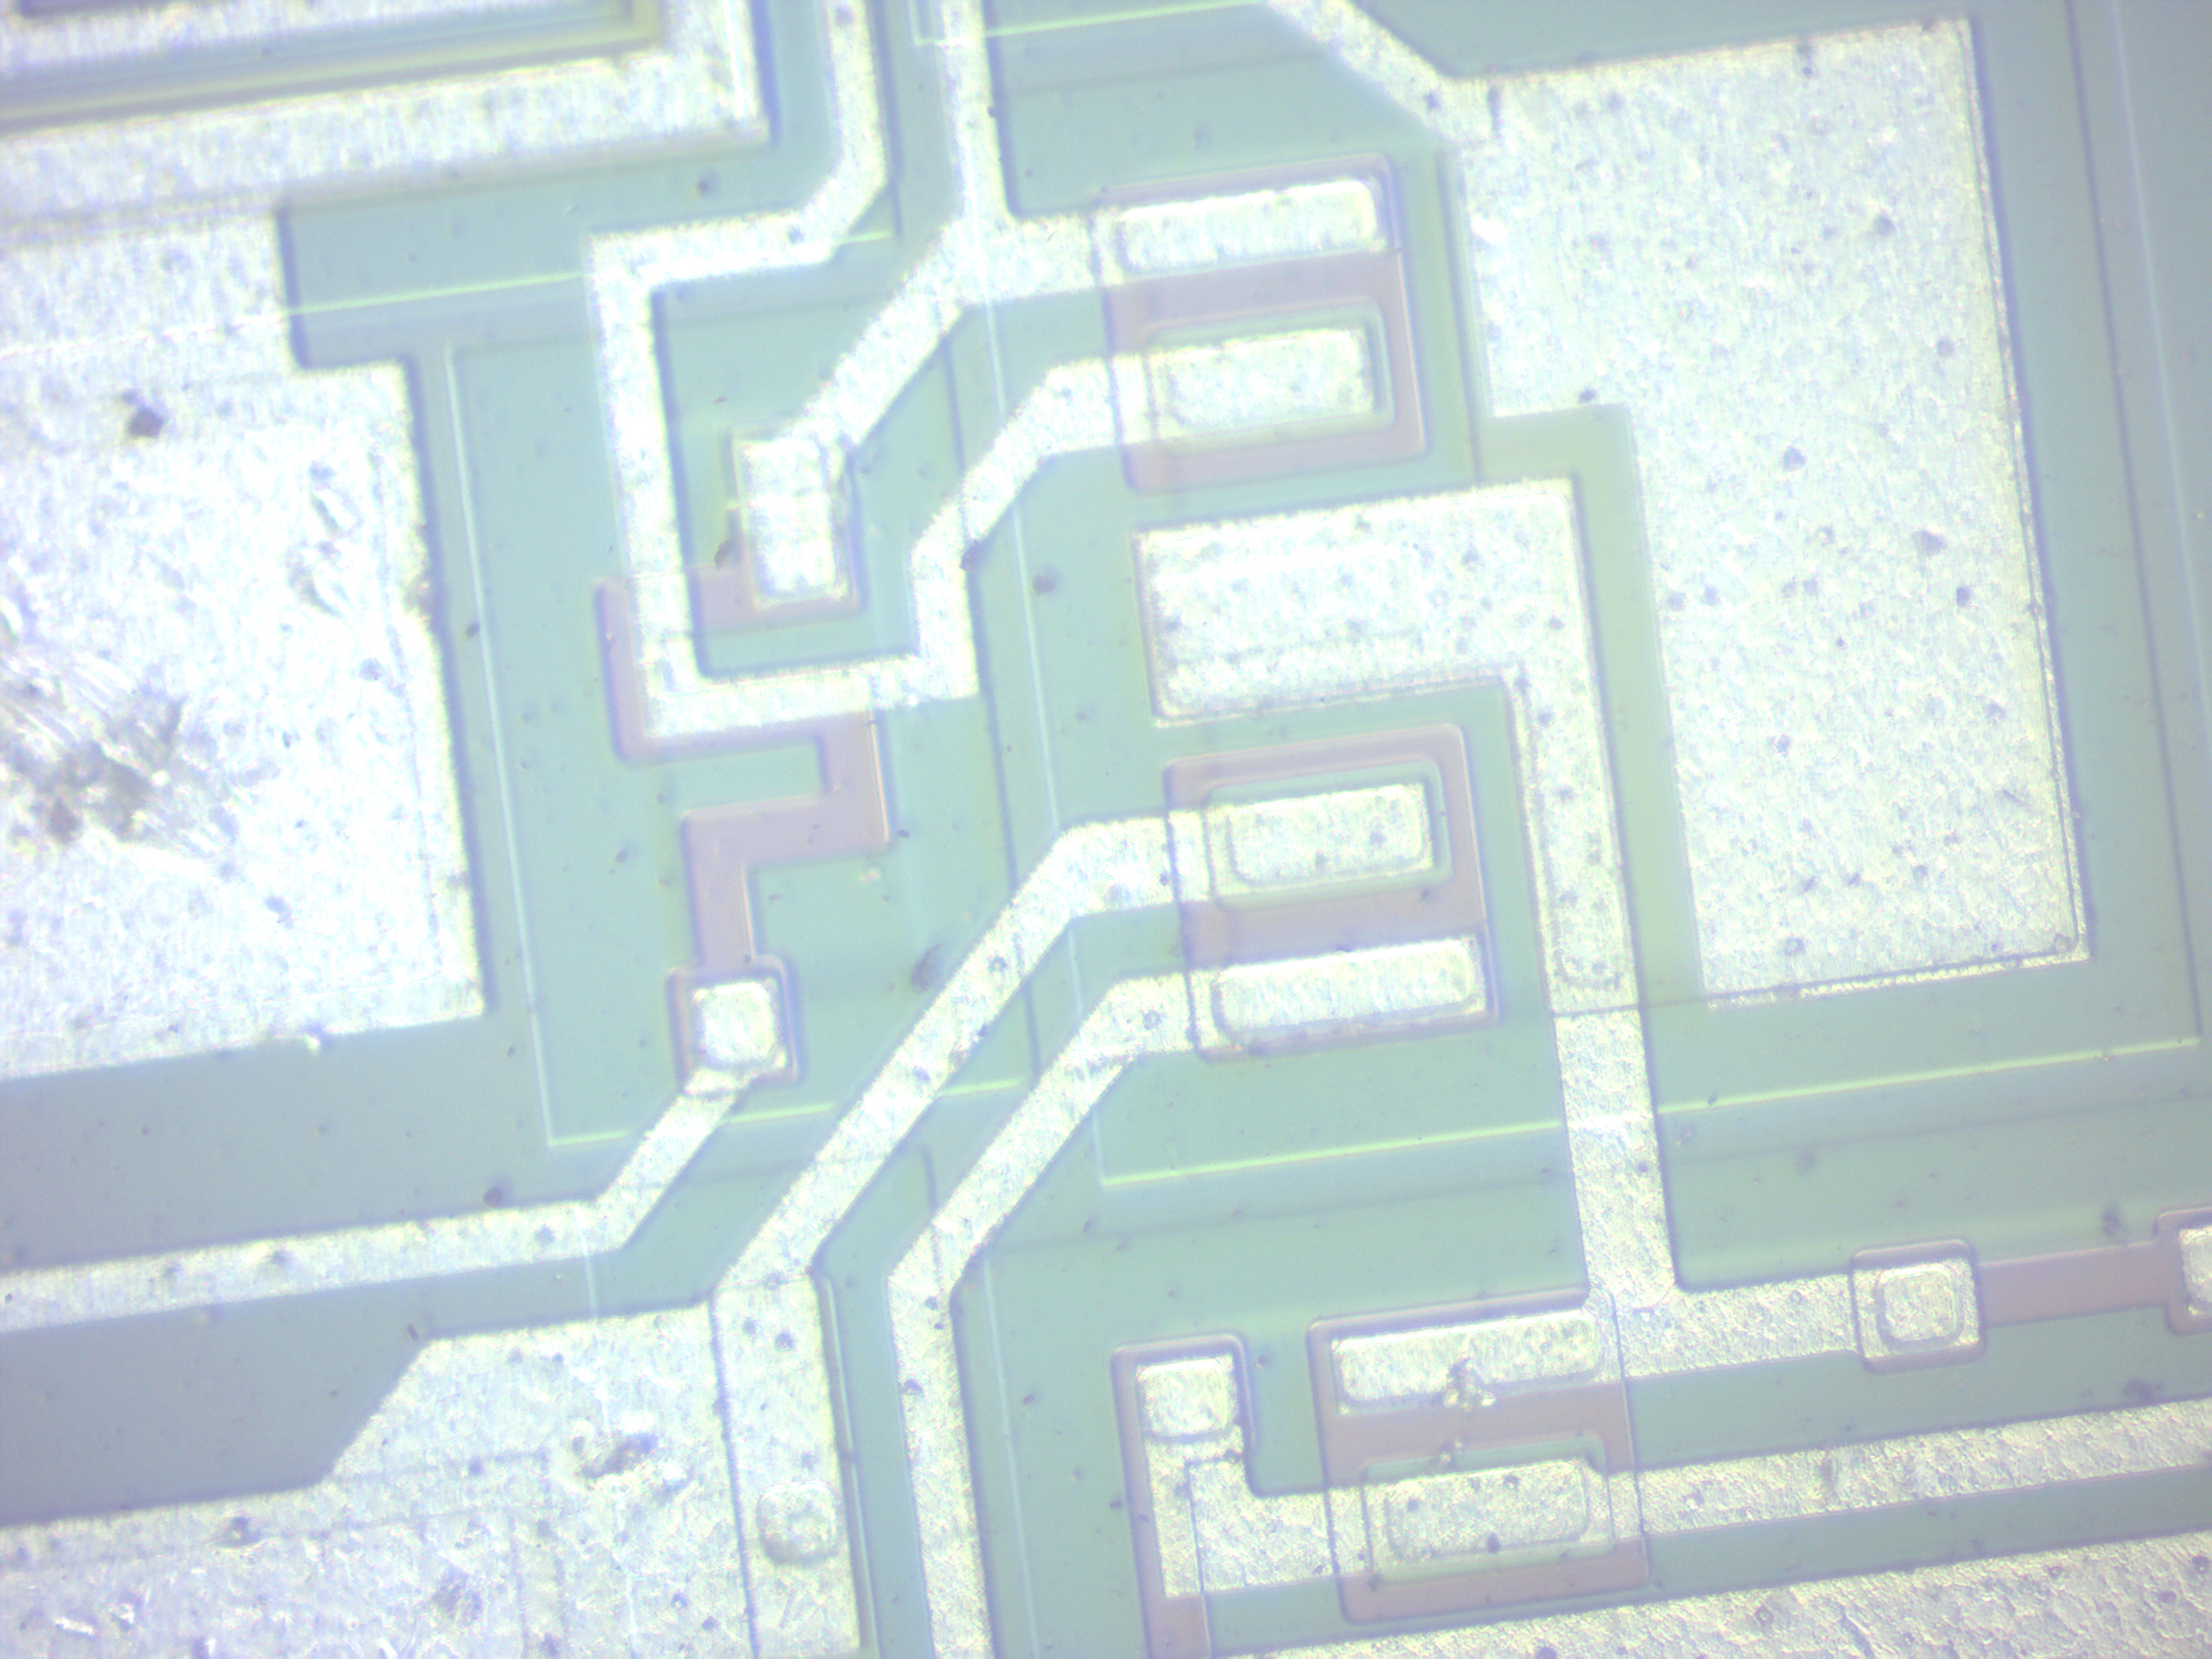
\includegraphics[width=0.7\linewidth]{./figures/microscope/Chip}

}

\caption{Close-up view of an electronic chip.}\label{fig:chip}
\end{figure}

\begin{figure}

{\centering 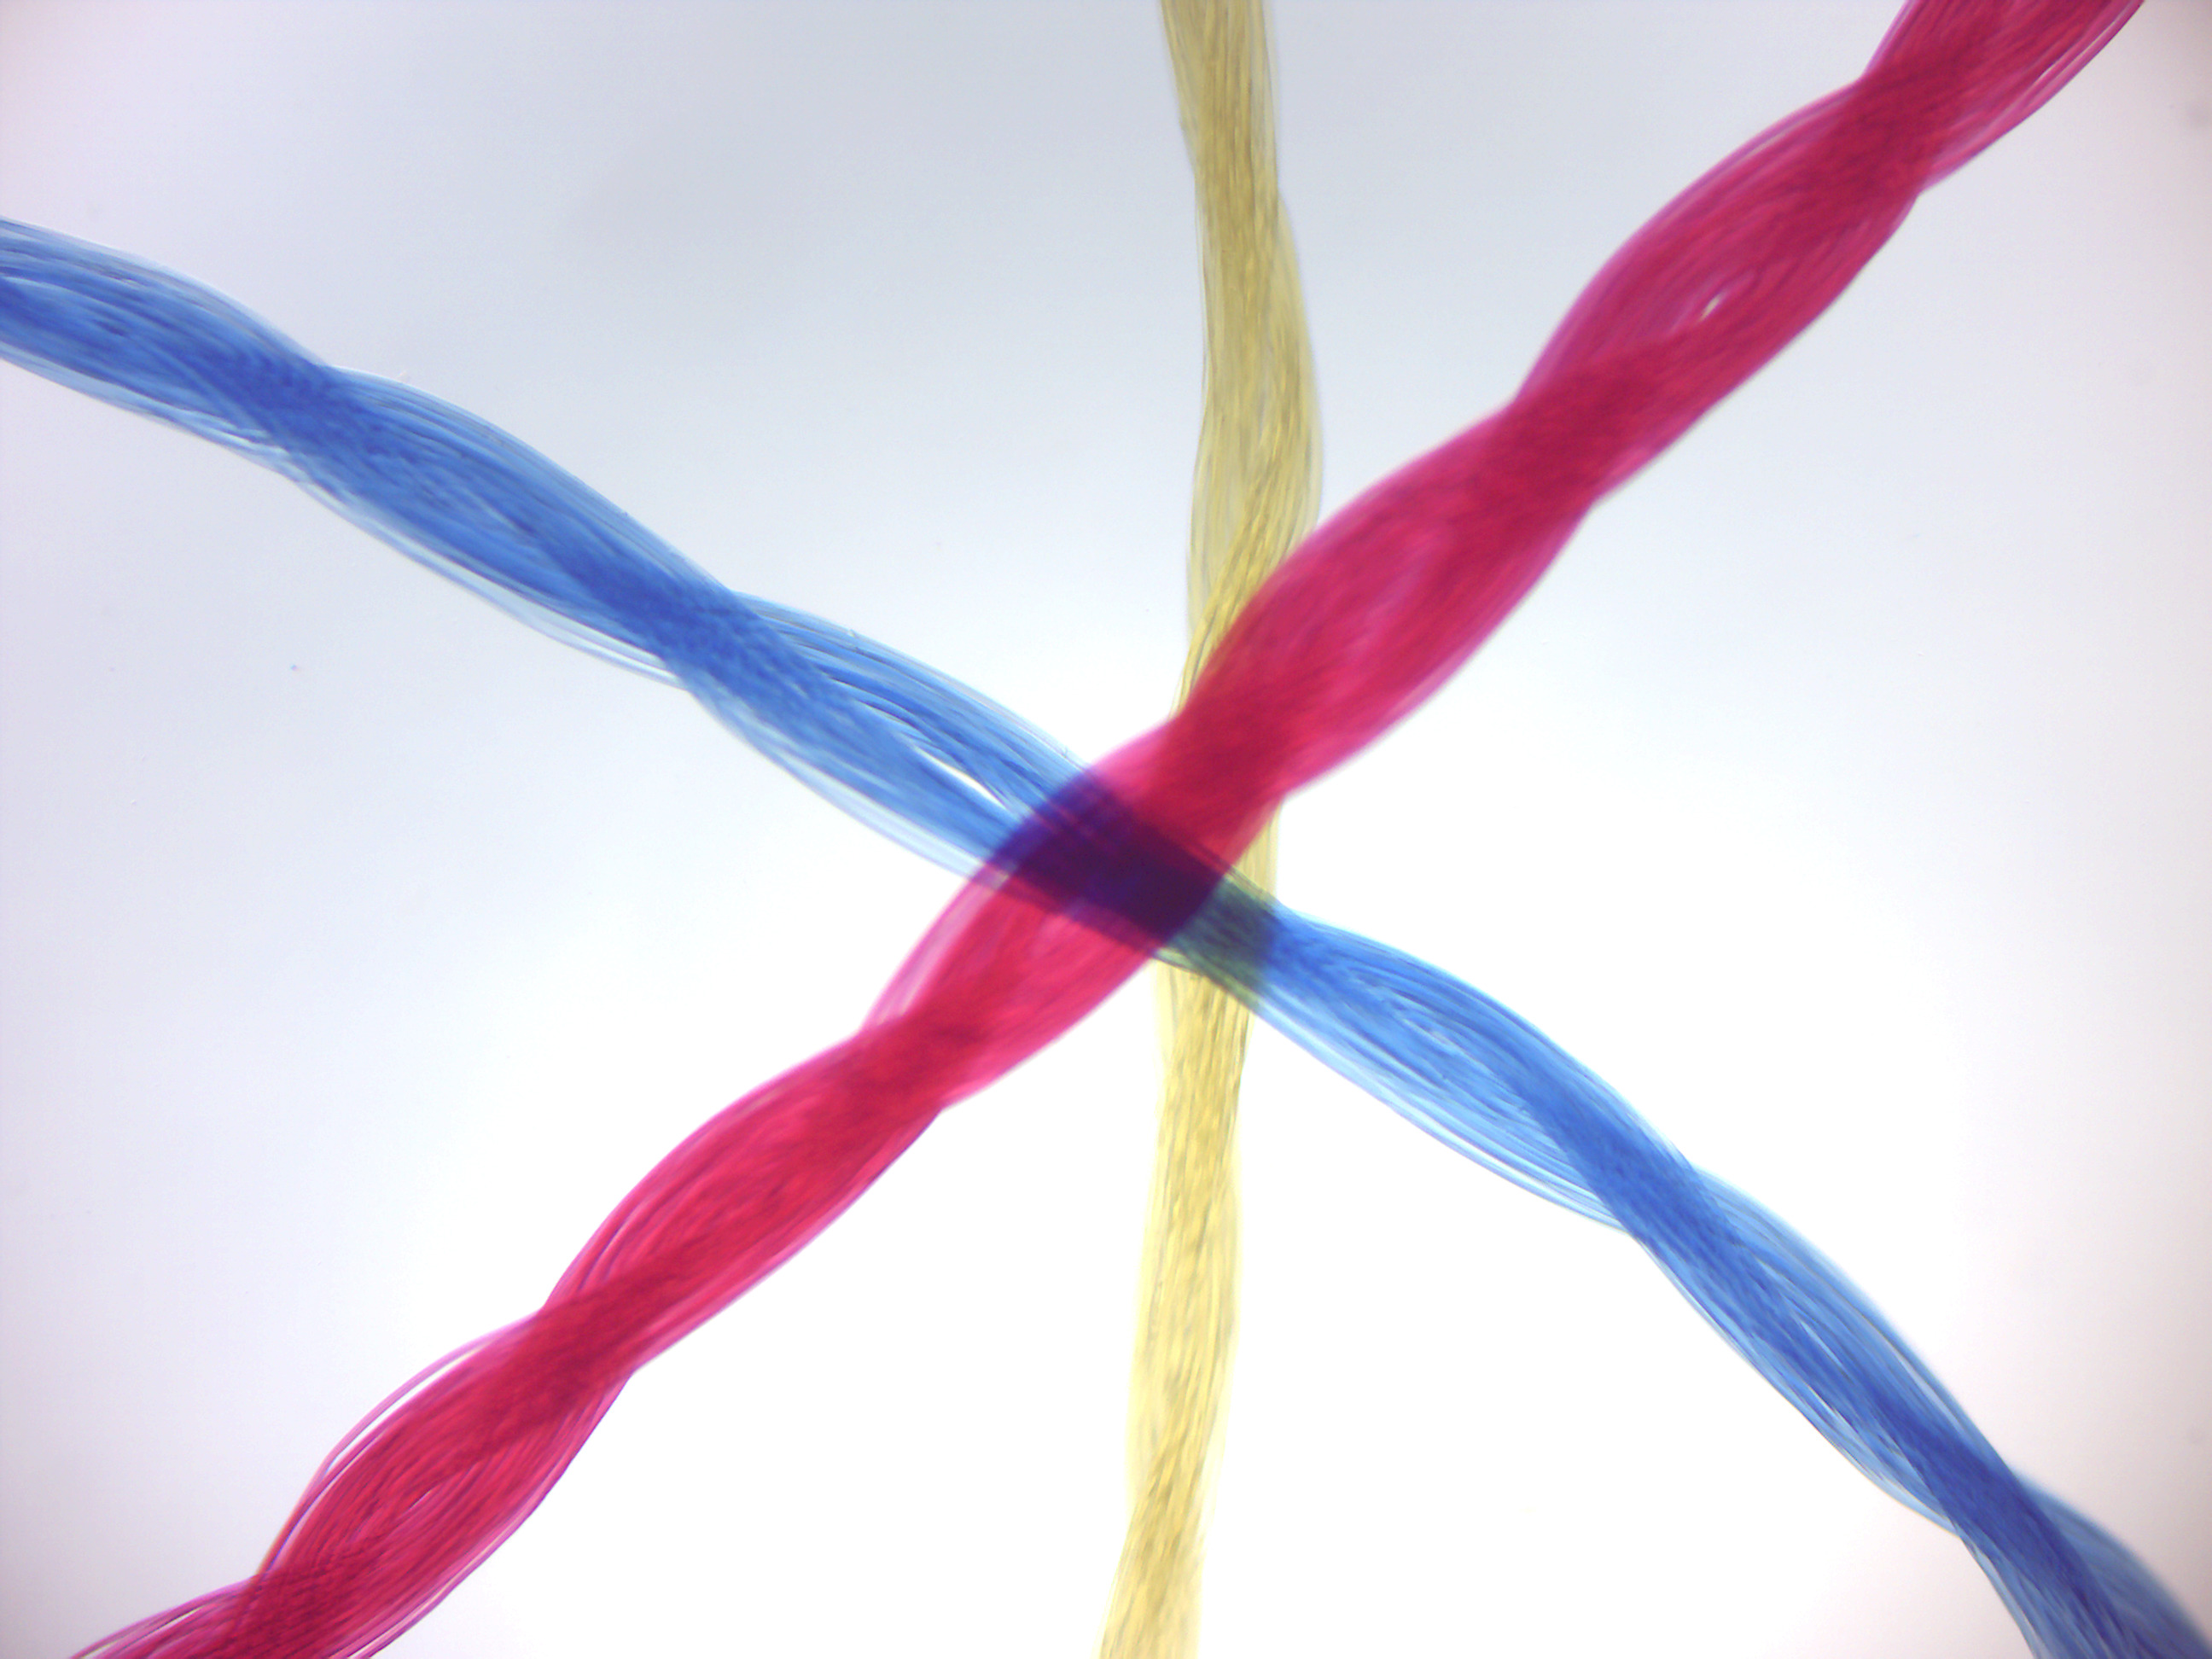
\includegraphics[width=0.7\linewidth]{./figures/microscope/Threads}

}

\caption{Which thread is on top, in the middle, at the bottom?}\label{fig:threads}
\end{figure}

\begin{figure}

{\centering 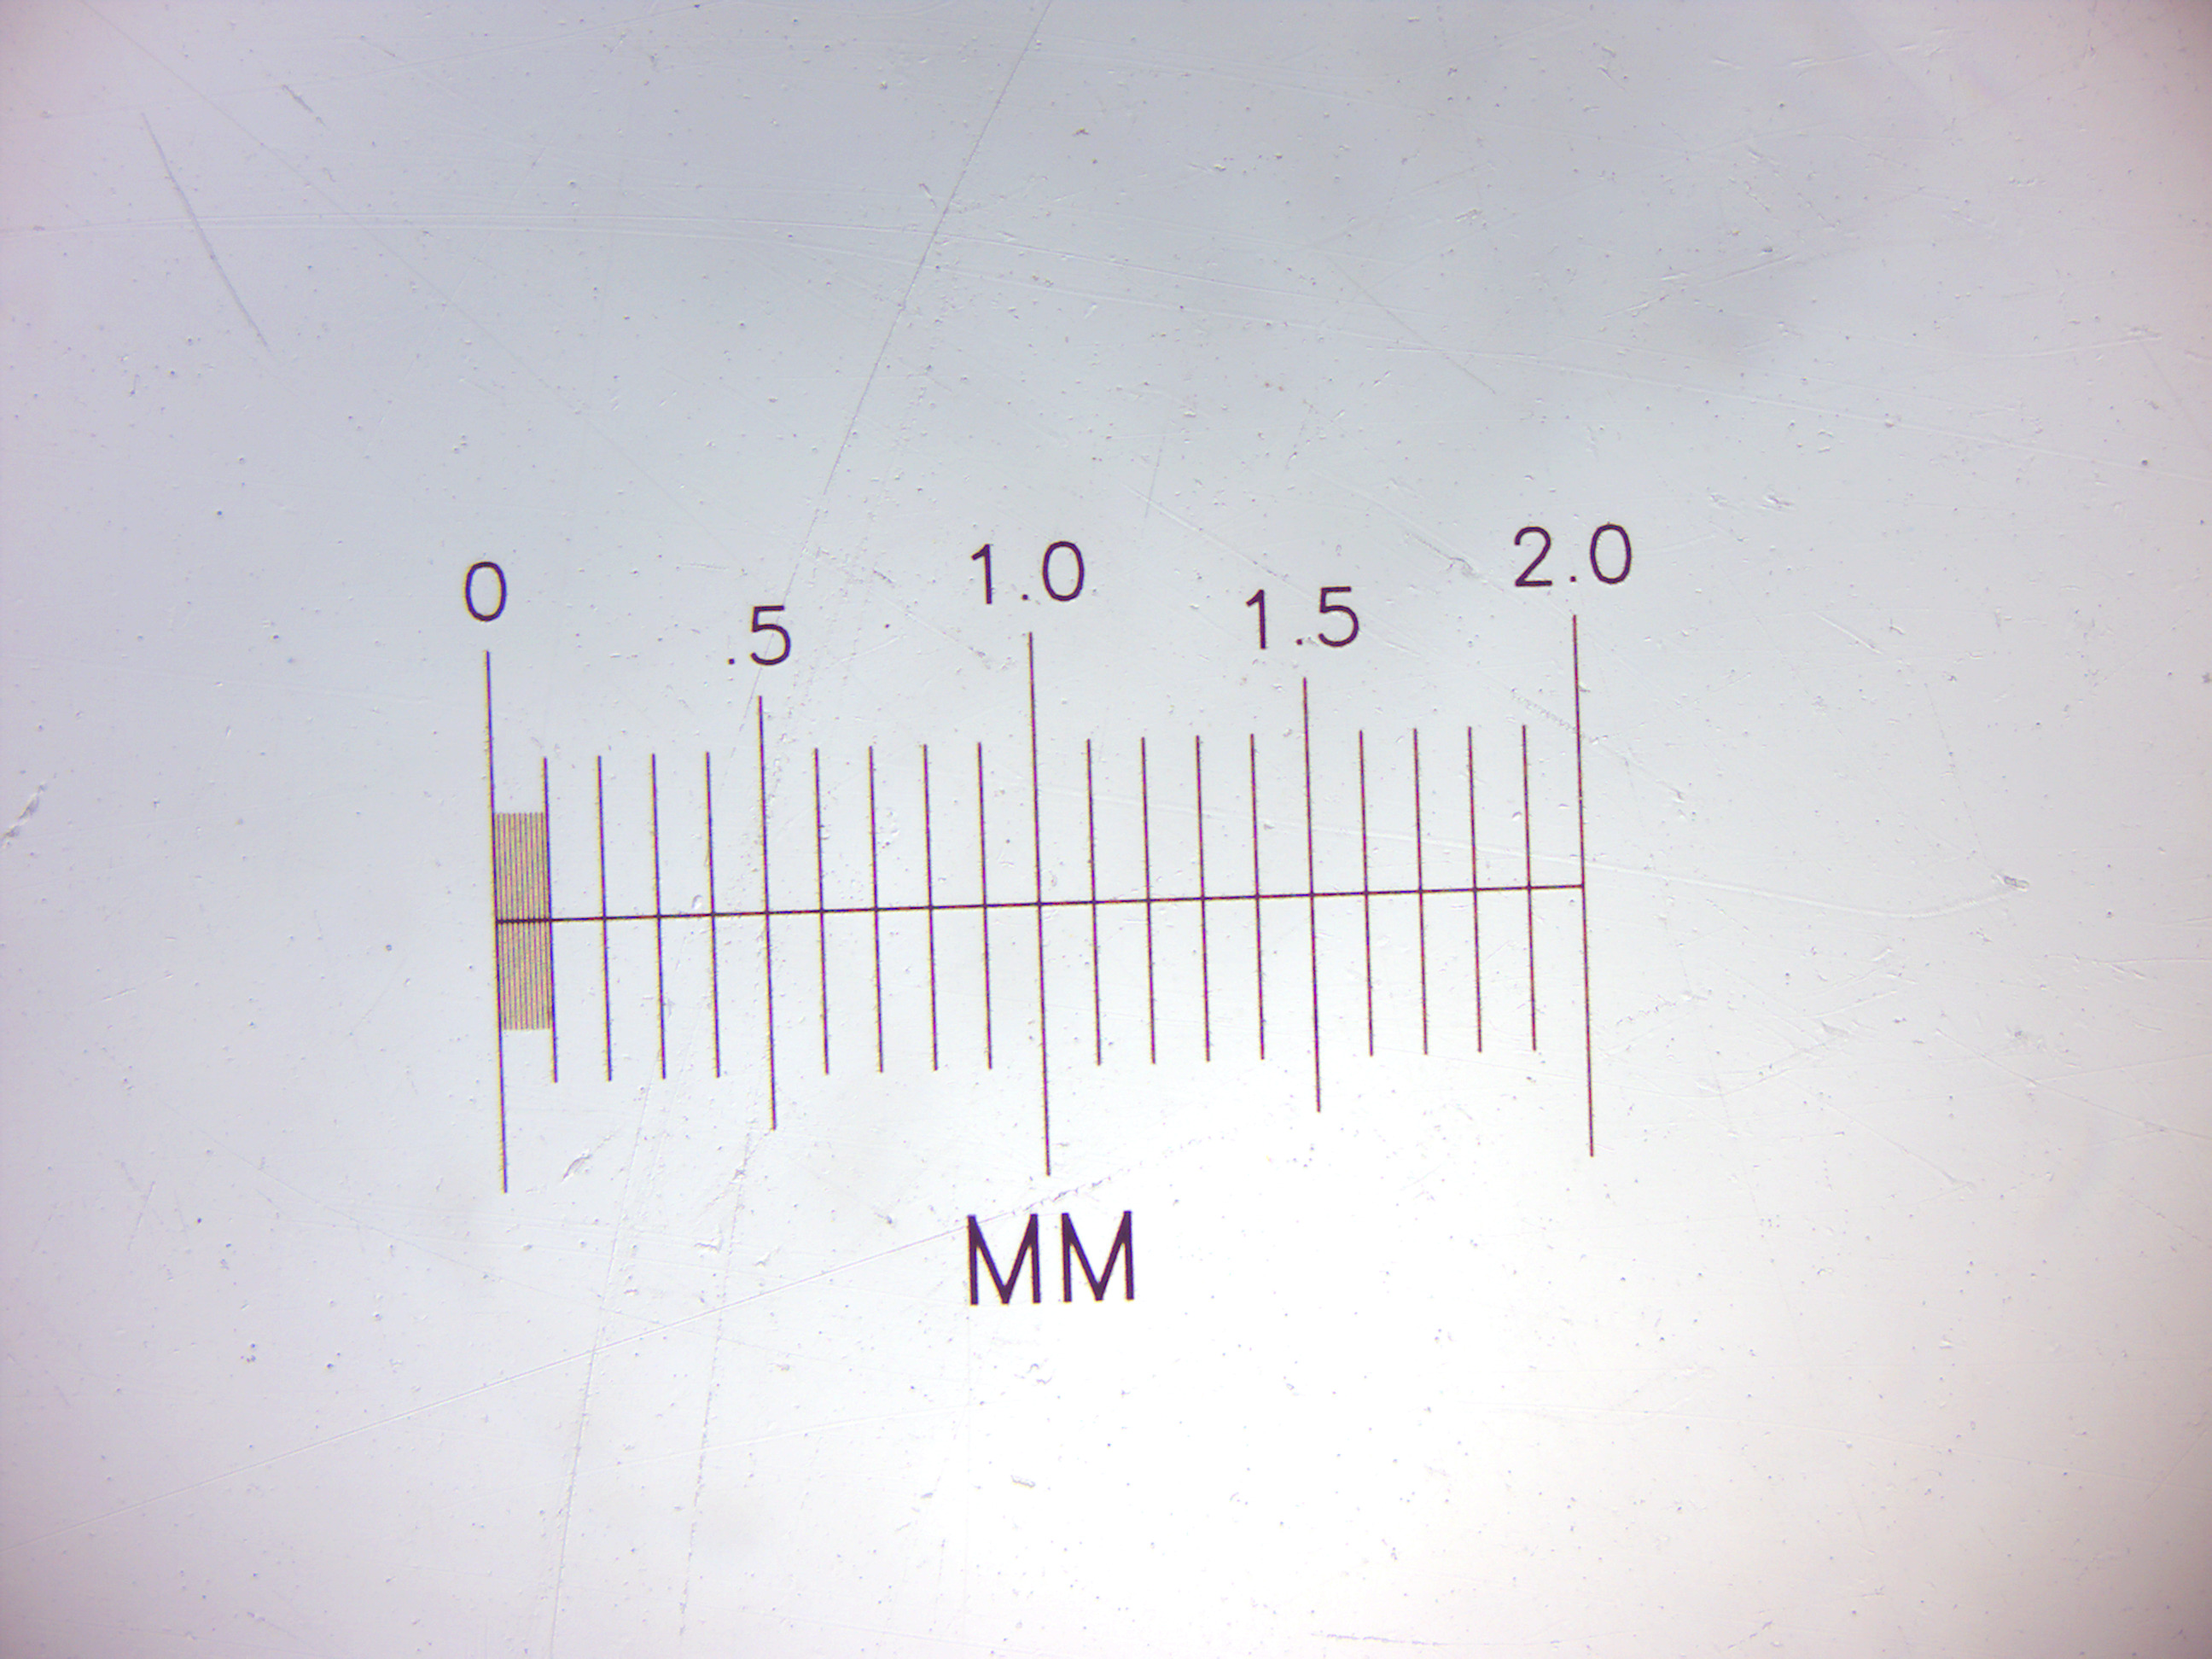
\includegraphics[width=0.7\linewidth]{./figures/microscope/MM_scale}

}

\caption{A microscopic scale.}\label{fig:scale}
\end{figure}

\begin{figure}

{\centering 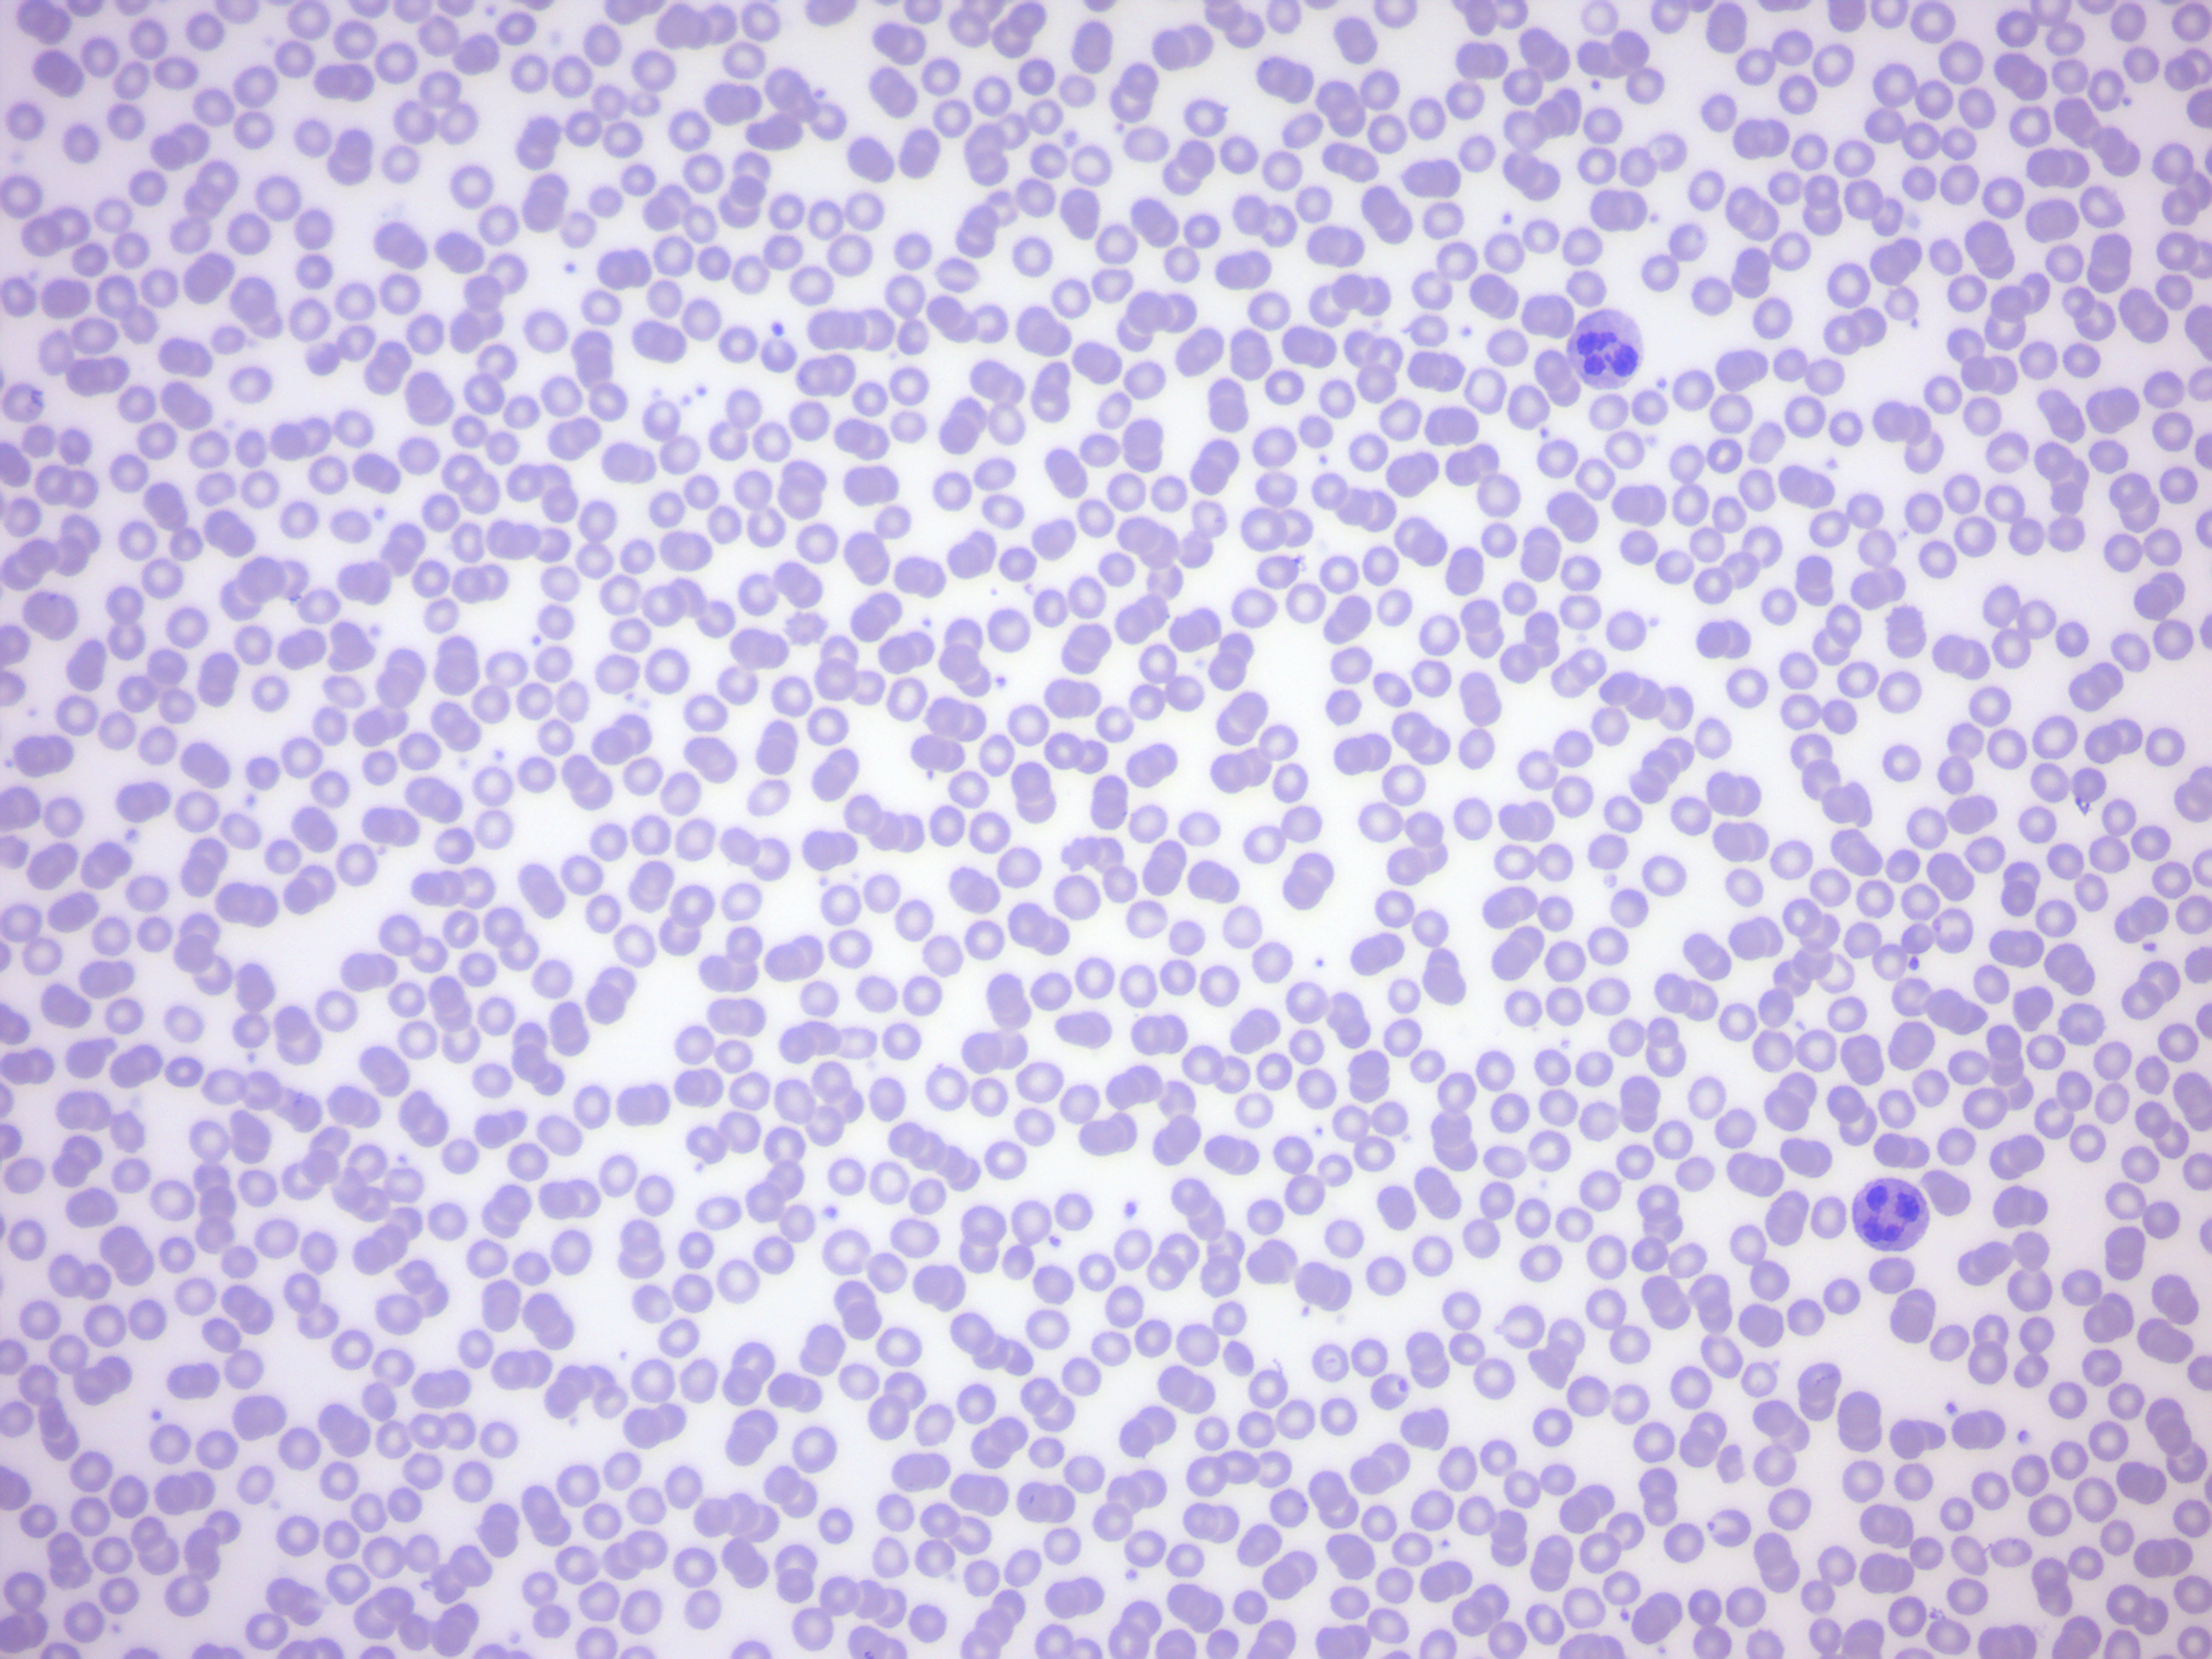
\includegraphics[width=0.7\linewidth]{./figures/microscope/Blood_smear}

}

\caption{A human blood smear.}\label{fig:smear}
\end{figure}

\section{Elodea Leaf Wet Mount}\label{elodea-leaf-wet-mount}

\href{https://en.wikipedia.org/wiki/Elodea_canadensis}{\emph{Elodea
canadensis}} (American or Canadian waterweed or pondweed) is a perennial
aquatic plant, or submergent macrophyte, native to most of North
America. It grows rapidly in favorable conditions and can choke shallow
ponds, canals, and the margins of some slow-flowing rivers. It requires
summer water temperatures of 10-25 °C and moderate to bright lighting.
Young plants initially start with a seedling stem with roots growing in
mud at the bottom of the water; further adventitious roots are produced
at intervals along the stem, which may hang free in the water or anchor
into the bottom. It grows indefinitely at the stem tips, and single
specimens may reach lengths of 3 m or more. The leaves are bright green,
translucent, oblong, 6-17 mm long and 1-4 mm broad, borne in whorls of
three (rarely two or four) round the stem. It lives entirely underwater,
the only exception being the small white or pale purple flowers which
float at the surface and are attached to the plant by delicate stalks.
It is dioecious, with male and female flowers on different plants. The
flowers have three small white petals; male flowers have 4.5-5 mm petals
and nine stamens, female flowers have 2-3 mm petals and three fused
carpels. The fruit is an ovoid capsule, about 6 mm long containing
several seeds that ripen underwater. The seeds are 4-5 mm long,
fusiform, glabrous (round), and narrowly cylindrical. It flowers from
May to October.

\subsection{Experimental procedures}\label{experimental-procedures}

\begin{enumerate}
\def\labelenumi{\arabic{enumi}.}
\tightlist
\item
  Get a single leaf from the Elodea plant and mount it on a slide, cover
  it with a drop of water and a cover slip.
\item
  Place the slide onto the microscope state and observe at the leaf
  under the microscope.
\item
  These leaves are two cells thick, so you should be able to focus up
  and down to see that the cells in one layer are larger than those in
  the other. When one layer is in focus, you may be able to see the
  shadowy outlines of cell walls in the other layer.
\item
  Notice that the cells are clearly delineated by the cell wall.
\item
  Inside the cells are large oval-shaped green bodies, the chloroplasts.
\item
  As the cells warm, you can see the chloroplasts carried by the moving
  cytoplasm around the nearly transparent nucleus in the center of the
  cell.
\item
  Make a drawing of what you see at 400× magnification.
\end{enumerate}


\begin{figure}

{\centering 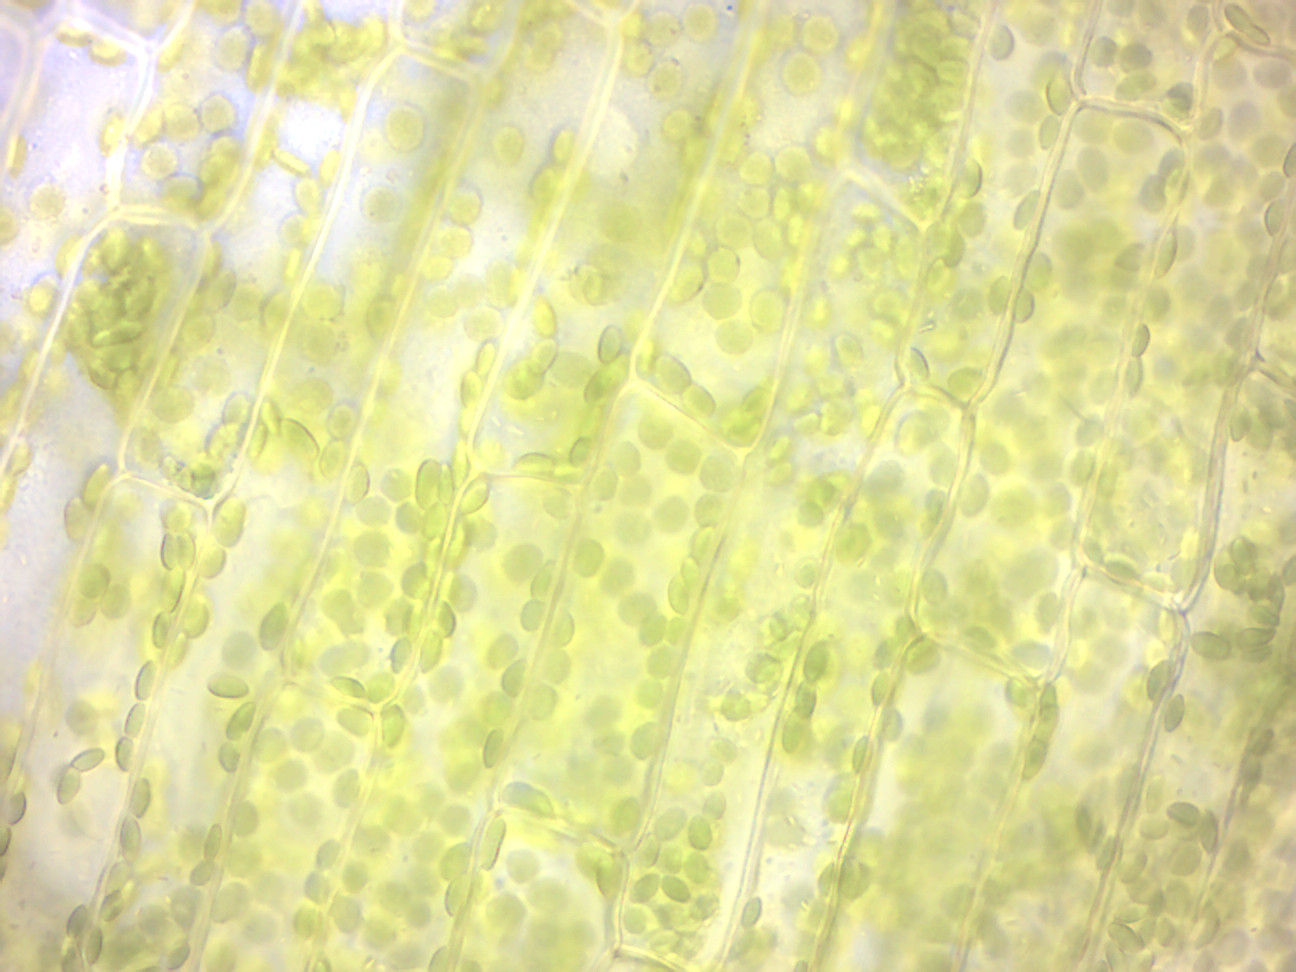
\includegraphics[width=0.7\linewidth]{./figures/microscope/elodea}

}

\caption{Elodea wet mount at 1000× magnification.}\label{fig:elodea}
\end{figure}


\section{How to turn off the
microscope}\label{how-to-turn-off-the-microscope}

The tablets and microscopes must be turned off in a specific order:

\begin{enumerate}
\def\labelenumi{\arabic{enumi}.}
\tightlist
\item
  Turn off microscope using the switch on the lower right side.
\item
  While the microscope is still plugged in, turn off the tablet by
  holding the power button down for a few seconds. Select power off.
\item
  Motic logo will appear on tablet.
\item
  Wait till charging symbol will appear.
\item
  Leave microscopes kept on the student bench plugged in after turning
  them off and place the cover over the microscope.
\end{enumerate}

\section{Review Questions}\label{review-questions}

\begin{enumerate}
\def\labelenumi{\arabic{enumi}.}
\tightlist
\item
  Why do biologists use microscopes?
\item
  What is the function of the microscope objectives?
\item
  What are the magnification factors of the objectives of our
  microscopes?
\item
  What is the name of the lenses that are close to your eyes when you
  look through the microscope?
\item
  What is the magnifying power of these lenses?
\item
  What is the total magnification of the image that you observe if you
  use the 40× objective?
\item
  What is the difference between the action of the coarse and the fine
  focus knobs?
\item
  Which part of the microscope moves when you turn the focus knobs?
\item
  What is the field of view?
\item
  How does it change when you switch from a lower to a higher power
  objective?
\end{enumerate}
